\documentclass[12pt]{article}

% ─── Packages ─────────────────────────────────────────────────────────────────
\usepackage[a4paper, margin=2.54cm, headheight=14pt]{geometry}
\usepackage{setspace}
\usepackage{times}
\usepackage{amsmath, amssymb}
\usepackage{booktabs}
\usepackage{array}
\usepackage{graphicx}
\usepackage{hyperref}
\usepackage[numbers,sort&compress]{natbib}
\usepackage{fancyhdr}
\usepackage{titlesec}
\usepackage{microtype}
\usepackage[T1]{fontenc}
\usepackage[utf8]{inputenc}
\usepackage{caption}
\usepackage{float}
\usepackage{algorithm}
\usepackage{algpseudocode}

% ─── Spacing & Layout ─────────────────────────────────────────────────────────
\doublespacing
\setlength{\parindent}{0.5in}
\setlength{\parskip}{0pt}

% ─── Header / Footer ──────────────────────────────────────────────────────────
\pagestyle{fancy}
\fancyhf{}
\rhead{\small\MakeUppercase{Permutation Test for Menstrual Cycle Regularity Counts}}
\rfoot{\thepage}
\renewcommand{\headrulewidth}{0pt}

% ─── Section formatting ───────────────────────────────────────────────────────
\titleformat{\section}{\normalfont\normalsize\bfseries}{\thesection.}{0.5em}{}
\titleformat{\subsection}{\normalfont\normalsize\bfseries}{\thesubsection}{0.5em}{}
\titleformat{\paragraph}[runin]{\normalfont\normalsize\bfseries}{}{0pt}{}[\ ---]
\titlespacing*{\section}{0pt}{12pt}{6pt}
\titlespacing*{\subsection}{0pt}{10pt}{4pt}
\titlespacing*{\paragraph}{0pt}{6pt}{0.5em}

% ─── Hyperlink styling ────────────────────────────────────────────────────────
\hypersetup{colorlinks=true, linkcolor=blue, citecolor=blue, urlcolor=blue}

% ─── Table column types ───────────────────────────────────────────────────────
\newcolumntype{L}[1]{>{\raggedright\arraybackslash}p{#1}}
\newcolumntype{C}[1]{>{\centering\arraybackslash}p{#1}}

% ─── Figure path ──────────────────────────────────────────────────────────────
\graphicspath{{figures/}}
\captionsetup{font=small, labelfont=bf, width=0.92\textwidth}

% ══════════════════════════════════════════════════════════════════════════════
\begin{document}

% ─── Title Page ───────────────────────────────────────────────────────────────
\begin{titlepage}
  \centering
  \vspace*{3cm}
  {\large\bfseries A Multivariate Permutation Test for Correlated Menstrual Cycle Regularity Counts:\\[4pt]
  \normalfont\large Application to Jewish Halachic Anticipatory Rules\par}
  \vspace{1.5cm}
  {[Author details removed for peer review]\par}
  \vspace{3cm}
  {\normalsize\bfseries Author Note\par}
  \vspace{0.5cm}
  \begin{flushleft}
  [Author details removed for peer review]

  \medskip
  The dataset analyzed in this study was originally collected by
  Fehring et al.~\cite{fehring2013} and is publicly archived at Marquette
  University \cite{marquette2013data}. The author declares no conflicts of interest.
  Analysis code is publicly available at \url{https://[URL removed for peer review]}.

  \medskip
  Correspondence: [removed for peer review]
  \end{flushleft}
\end{titlepage}

% ─── Abstract ─────────────────────────────────────────────────────────────────
\newpage
\begin{center}{\bfseries Abstract}\end{center}

\noindent
Jewish religious law (\textit{Halacha}) prescribes that women anticipate menstruation
based on recurring patterns in their cycle history. These anticipatory rules are
the \textit{halachic vesset rules} (\textit{vesset}: Hebrew for menstruation).
Five testable vesset rule types involve cycle-length data: \textit{Haflaga} (fixed interval),
\textit{Dilug} (arithmetic progression), \textit{Week} (weekly anchor),
\textit{Week-Dilug} (30-day anchor), and \textit{Dilug-in-Dilug} (second-order
progression). These form a polynomial hierarchy with algebraic containment and
approximation relationships; pairwise rate-based Spearman correlations confirm
inter-pattern association (Haflaga $\times$ Dilug-in-Dilug: $r_s = 0.27$,
Holm-adj $p = .030$).
We apply three complementary null models to 1,554 menstrual cycles from 118 women
\cite{fehring2013}: a global permutation null, a multinomial sampling null, and a
within-woman permutation null conditioning on each woman's observed
cycle-length multiset. Under the global null, \textit{Haflaga} is strongly
overrepresented ($z = 4.51$, $p < .001$); a 5-pattern Mahalanobis joint test
detects significant multivariate departure ($D_M = 5.10$, $p < .001$),
reflecting concentration of patterns among women with lower cycle-length variability.
Under the within-woman null --- the scientifically sharper test --- no pattern
is significant (all Holm-corrected $p \geq .198$; joint $D_M = 2.95$, $p = .121$), and all observed
counts fall \emph{below} their within-woman null means (all below the normal-theory
minimum detectable count; Table~\ref{tab:power}), indicating limited sensitivity. These complementary results
suggest that halachic vesset rules function primarily as empirical detectors of
individual cycle regularity, with no detectable evidence, under within-woman exchangeability,
that temporal ordering adds structure beyond each woman's own cycle-length distribution.

\medskip
\noindent\textit{Keywords:} menstrual cycle, vesset, Halacha, permutation test,
within-woman permutation, multinomial sampling, natural family planning, Jewish law,
polynomial hierarchy, dependence structure, multivariate randomization test

% ─── 1. Introduction ──────────────────────────────────────────────────────────
\newpage
\section{Introduction}

Menstrual cycles exhibit substantial variability both within and across individuals
\cite{munster1992,creinin2004,symul2019}. The cycle length distribution is
approximately bell-shaped with a pronounced right tail (skewness $\approx 1.3$ in the
present dataset), reflecting a small proportion of unusually long cycles. Within-person
consistency is moderate: intraclass correlation coefficients for cycle length are
typically in the range of $0.3$--$0.5$ \cite{dasharathy2012}, indicating meaningful
regularity beneath the surface variability. Bayesian hierarchical state-space models have
been proposed to exploit this temporal structure for cycle-length prediction
\cite{bortot2010}, confirming that within-woman dynamics carry genuine predictive
information.

In the Jewish religious tradition, this regularity is also subject to detailed legal
analysis. Halachic law (\textit{Halacha}, Jewish religious law) requires that a woman anticipate the onset of
her next menstruation based on patterns discernible in her prior cycle history. These
anticipatory rules --- the \textit{halachic vesset rules} --- govern a system of abstinence
obligations central to the observance of \textit{taharat hamishpacha} (family purity: the traditional Jewish
system of laws governing marital intimacy in relation to the menstrual cycle). Of the 17 vesset pattern types documented in halachic literature, 10 require
date or time-of-day data unavailable in standard cycle-length records; the remaining
7 are testable empirically. Two of these 7 (Dilug Chozer Chalila and Haflaga Chozer Chalila
(Hebrew: repeating-cycle arithmetic progression and repeating fixed interval,
respectively) occurred zero times in the present dataset and are not reported separately.
The five patterns with positive observed frequencies are analysed here.

These five patterns form a \textit{polynomial hierarchy}: each describes a \textit{haflaga} (Hebrew: inter-menstrual interval, $H_k = L_k + 1$)
sequence that follows a polynomial of a specific degree in cycle index. Haflaga,
Week, and Week-Dilug are all degree-0 (constant) sequences; Dilug is degree-1
(linear); Dilug-in-Dilug is degree-2 (quadratic). This hierarchy generates
algebraic structural relationships between the patterns --- one of which
(Haflaga-30 $\subseteq$ Week-Dilug) is a strict logical containment, and
another (Haflaga--Dilug-in-Dilug proximity) an algebraic approximation rather
than a logical implication --- with implications for how their joint frequencies
should be tested.

Despite the centuries-long practical application of vesset rules --- and the modern
availability of large longitudinal cycle datasets --- no published study has formally
tested whether these patterns occur in empirical data at rates exceeding chance. This
is a non-trivial question: if vesset rules merely detect random fluctuations, their
anticipatory validity is weakened. Conversely, if they depart significantly from chance expectations,
their empirical basis is independently corroborated.

The present study addresses this gap by applying two complementary null models ---
a permutation test \cite{edgington2007} and a multinomial sampling null
\cite{anon2022phd} --- to a longitudinal NFP dataset \cite{fehring2013}. We derive
per-pattern p-values, effect sizes, and a joint multivariate test that accommodates
the dependence structure among pattern counts without assuming independence. The joint
test represents a methodological contribution \cite{anon2022phd}, inspired by the
simulation-based testing philosophy of King et al.\ \cite{king2018} though distinct
from their density-based approach; related ideas appear in multivariate permutation
tests using quadratic forms \cite{pesarin2010}; a formal theoretical treatment is
planned in future work. We also characterise the mathematical dependence structure through pairwise
rate-based Spearman correlation tests and derive the dependencies analytically from the pattern definitions.

This study extends a line of quantitative halachic scholarship \cite{anon2022markov,
anon2019reliability,anon2021statistical}. To our knowledge it is the first to test vesset pattern frequencies against
an explicit randomisation null, though we note this claim has not been verified
by a systematic literature search.

% ─── 2. Background ────────────────────────────────────────────────────────────
\section{Background}

\subsection{The Polynomial Hierarchy of Vesset Rules}

Let $L_1, L_2, \ldots, L_n$ denote the menstrual cycle lengths (in days) of a single
woman, and define the \textit{haflaga} $H_k = L_k + 1$ (the interval from the first
day of menstruation $k$ to the first day of menstruation $k+1$, following halachic
convention \cite{anon2021statistical}). The five vesset pattern types are:

\begin{description}
  \item[\textit{Haflaga.}] $H_k = H_{k-1} = H_{k-2}$ (three or more consecutive
    equal haflaga values, any value). Degree-0 polynomial (constant, unrestricted).
    Minimum run: 3 cycles.

  \item[\textit{Dilug.}] $H_k - H_{k-1} = H_{k-1} - H_{k-2} = d \neq 0$ (constant
    non-zero first difference). Degree-1 polynomial (linear).
    Minimum run: 3 cycles.

  \item[\textit{Dilug-in-Dilug.}] $(H_k - H_{k-1}) - (H_{k-1} - H_{k-2}) =
    (H_{k-1} - H_{k-2}) - (H_{k-2} - H_{k-3}) = d \neq 0$ (constant non-zero second
    difference). Degree-2 polynomial (quadratic). Minimum run: 4 cycles.

  \item[\textit{Week.}] $H_k = H_{k-1}$, $H_k \in \mathcal{W}$ where
    $\mathcal{W} = \{H_{\min}+3, H_{\min}+10, \ldots\}$ (values spaced 7 apart,
    corresponding to the same weekday at each menstruation).
    Degree-0 polynomial anchored to weekly values. Minimum run: 2 cycles.

  \item[\textit{Week-Dilug.}] $H_k = H_{k-1} = 30$ (two or more consecutive haflaga values
    both equal to 30). The value $H = 30$ (29 actual days $= 4$ weeks $+ 1$ day) is
    the unique haflaga for which each successive menstruation falls one weekday later,
    producing an arithmetic progression of onset weekdays --- hence the name
    \textit{Week-Dilug} (Hebrew: \textit{shavu'a be-dilug}, week with arithmetic
    progression; \cite{anon2022phd}). Week-Dilug thus
    combines the constant-interval property of Haflaga with the arithmetic-progression
    concept of Dilug, applied to the weekday domain rather than the cycle-length domain.
    Degree-0 polynomial (constant) at the canonical 30-day anchor. Minimum run: 2 cycles.
\end{description}

The hierarchy Haflaga (degree 0) $\to$ Dilug (degree 1) $\to$ Dilug-in-Dilug
(degree 2) follows increasing polynomial order in cycle index. Week and Week-Dilug
are specialisations of the degree-0 case anchored to calendar values.

\subsection{Mathematical Dependence Structure}
\label{sec:mathdep}

The polynomial hierarchy generates two analytically derivable dependence
relationships between the remaining pattern pairs, which we verify empirically in
Section~\ref{sec:chisq}:

\paragraph{Haflaga and Dilug-in-Dilug --- proximity in the hierarchy.}
When the second difference $|d|$ of a Dilug-in-Dilug sequence is small, its first
differences are nearly equal and the haflaga sequence is nearly constant --- i.e.\
nearly a Haflaga. In the data, 16 of 27 observed DiD sequences have $|d| = 1$,
making them almost indistinguishable from a constant sequence. Both patterns further
share the same structural prerequisite: a minimum run of $\geq 3$ consecutive cycles
satisfying a regularity condition, selecting the same women with high within-person
cycle stability (within-person SD: Haflaga women $= 1.54$ days vs.\ no-vesset women
$= 3.17$ days).

\paragraph{Dilug and Week-Dilug --- logical incompatibility.}
Dilug requires $\Delta H_k \neq 0$ (strictly non-constant differences); Week-Dilug
requires $H_k = H_{k-1} = 30$ ($\Delta H = 0$). These conditions are mutually
exclusive within the same cycle window, creating a negative dependence tendency.

\subsection{Prior Work}

\paragraph{Menstrual cycle statistics.}
Variability and regularity of cycle length have been extensively characterised
\cite{munster1992,creinin2004,dasharathy2012,symul2019}. Bortot et al.\
\cite{bortot2010} developed a Bayesian hierarchical state-space model for sequential
prediction of cycle lengths, exploiting within-woman temporal dependence; their model
provides a benchmark for cycle-length predictability.

\paragraph{Quantitative halachic analysis.}
Ross \cite{anon2022markov} modelled cycle transitions with Markov chains;
\cite{anon2019reliability} evaluated reliability of self-reported menstrual data in
a halachic context; \cite{anon2021statistical} applied statistical analysis to
abstinence laws. The present study applies a formal permutation-based hypothesis test to ask whether
vesset patterns occur at rates distinguishable from chance in real data --- to our
knowledge the first such test applied to this specific domain.

\paragraph{Cycle-length autocorrelation and dataset overlap.}
Ecochard et al.\ \cite{ecochard2024} provide evidence that the ovarian cycle is
driven by an internal circamonthly oscillator, using multi-cohort longitudinal data
that includes a North American dataset collected by Fehring and Schneider --- two of
whom are co-authors on both that study and the dataset analysed here
\cite{fehring2013}. The Marquette cohort used in Ecochard et al.\ (1,649 cycles,
159 women) is likely drawn from the same data-collection infrastructure as the
present dataset (1,554 cycles, 118 women after exclusion criteria); they are probably
not independent samples, though the exact overlap cannot be confirmed from the
archived data. The key methodological consequence is that second- to fourth-order
autocorrelation in cycle lengths --- documented in that cohort --- is expected to
be \emph{preserved} under $H_W$: permuting within each woman's sequence preserves
her observed cycle-length multiset, so any autocorrelation that merely modulates
cycle lengths within that multiset does not inflate the null distribution.
$H_W$ thus tests whether temporal \emph{ordering} produces additional exact vesset
events beyond what the observed cycle-length distribution would predict, regardless
of whether those lengths are autocorrelated.

\paragraph{Randomization-based testing.}
Permutation tests \cite{edgington2007,good2005} provide exact finite-sample p-values
under exchangeability. Exchangeability-block permutation --- permuting within groups
while preserving group structure --- is a well-established technique in neuroimaging
\cite{winkler2014,nichols2002} and is the statistical foundation of $H_W$ in the
present study. The multinomial sampling null \cite{anon2022phd} draws each
woman's cycles independently from the fitted empirical distribution, directly encoding
the null hypothesis of cycle independence. For the joint test, King et al.\
\cite{king2018} proposed a general framework for testing a vector of statistics via
simulation of the joint density, using a multivariate kernel density estimator to
define a smallest-acceptance-region test. The present joint test differs: we use the
Mahalanobis distance from the null mean vector as the test statistic, which is simpler,
requires no density estimation, and accounts for inter-pattern covariance. A formal
theoretical comparison is planned in future work \cite{anon2022phd}.

% ─── 3. Methods ───────────────────────────────────────────────────────────────
\section{Methods}
\label{sec:methods}

\subsection{Dataset}
\label{sec:data}

We analyzed a publicly available longitudinal dataset originally collected by Fehring
et al.\ \cite{fehring2013} in a randomised trial comparing two internet-supported
natural family planning methods, archived at Marquette University
\cite{marquette2013data}. After excluding cycles shorter than 18 days or longer than
54 days \cite{creinin2004}, the final sample comprised \textbf{1,554 cycles from 118
women} ($M = 13.2$ cycles per woman, $\text{SD} = 6.1$, range $5$--$45$).

Raw cycle lengths ranged from 18 to 54 days ($M = 29.3$, $\text{SD} = 3.9$,
$\text{Mdn} = 28.5$, skewness $= 1.29$). The distribution is approximately
bell-shaped with a right tail, consistent with the literature
\cite{munster1992,creinin2004}. Women ranged in age from 21 to 43 years
($M = 30.6$, $\text{SD} = 5.7$); parity data were not recorded in the archived
dataset. The dataset originates from two charting cohorts
($n_0 = 92$ and $n_1 = 67$ women in the raw data prior to exclusions;
$n_0 = 69$ and $n_1 = 49$ women in the filtered sample; cohort membership
was not used as a sensitivity variable in the primary analysis, though it is
available for future subgroup investigations). The minimum of 5 cycles
per woman in the analysed dataset reflects the observed minimum after the
cycle-length exclusion criteria were applied (18--54 days; complete records);
no additional minimum-cycle-count exclusion was imposed. All cycle lengths were incremented by 1 to conform to the
halachic haflaga convention ($H_k = L_k + 1$), yielding $M = 30.3$, $\text{SD} = 3.9$.

The within-person variability structure is relevant to the Haflaga result: women who
establish a Haflaga vesset ($n = 20$) have a mean within-person cycle-length SD of 1.54 days
(SD$_{\text{between}} = 0.59$), compared to 3.17 days (SD$_{\text{between}} = 1.75$) for women who
establish no vesset at all ($n = 35$). A Mann--Whitney test confirms this difference is highly
significant ($U = 133$, $p < .001$, two-sided; Welch $t = -5.05$, $\text{df} = 45.5$, $p < .001$;
95\% CI for mean difference: $[-2.29, -0.98]$ days; Cohen's $d = -1.13$). These results suggest that
Haflaga is associated with lower observed cycle-length variability. Note that within-person SD
estimates depend on the number of observed cycles per woman (dataset range: 5--45), so estimates
for women with few recorded cycles carry greater sampling uncertainty.
Figure~\ref{fig:dist} shows the cycle length distribution and per-woman variability.
Figure~\ref{fig:consort} summarises the data flow from source dataset to analysed sample.

\begin{figure}[H]
  \centering
  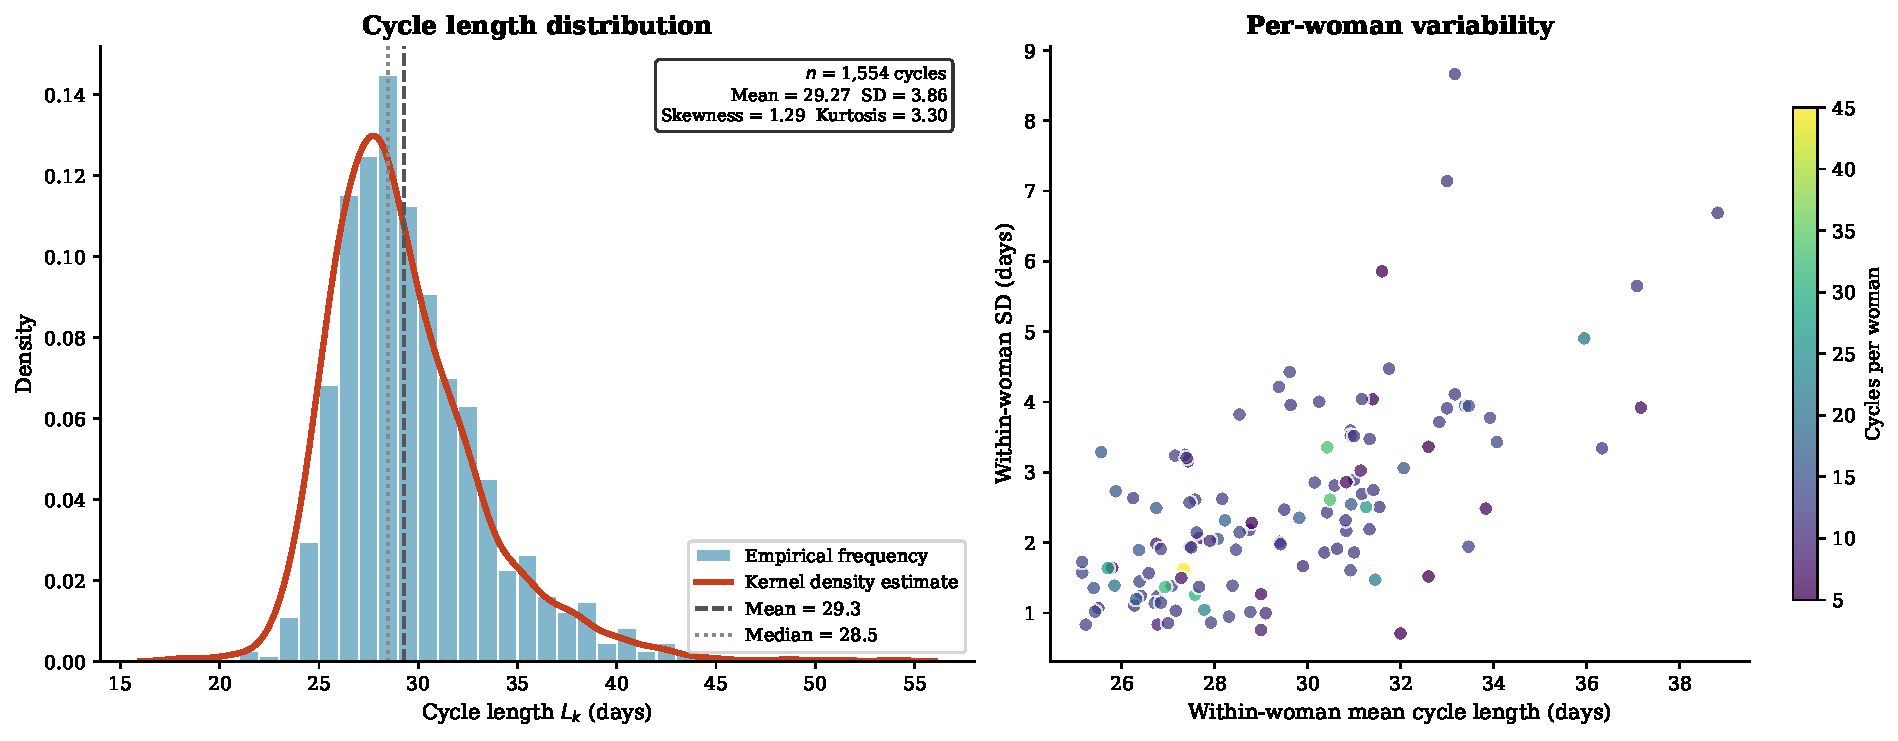
\includegraphics[width=\textwidth]{fig1_cycle_distribution}
  \caption{Cycle length distribution (filtered dataset). \textit{Left}: histogram
    and kernel density estimate of raw cycle lengths $L_k$, with mean (dashed) and
    median (dotted) marked. The distribution is right-skewed (skewness $= 1.29$).
    \textit{Right}: per-woman mean vs.\ within-person SD, shaded by cycle count.
    Women with more cycles tend to show lower variability, consistent with selection
    of naturally regular chartists.}
  \label{fig:dist}
\end{figure}

\begin{figure}[H]
  \centering
  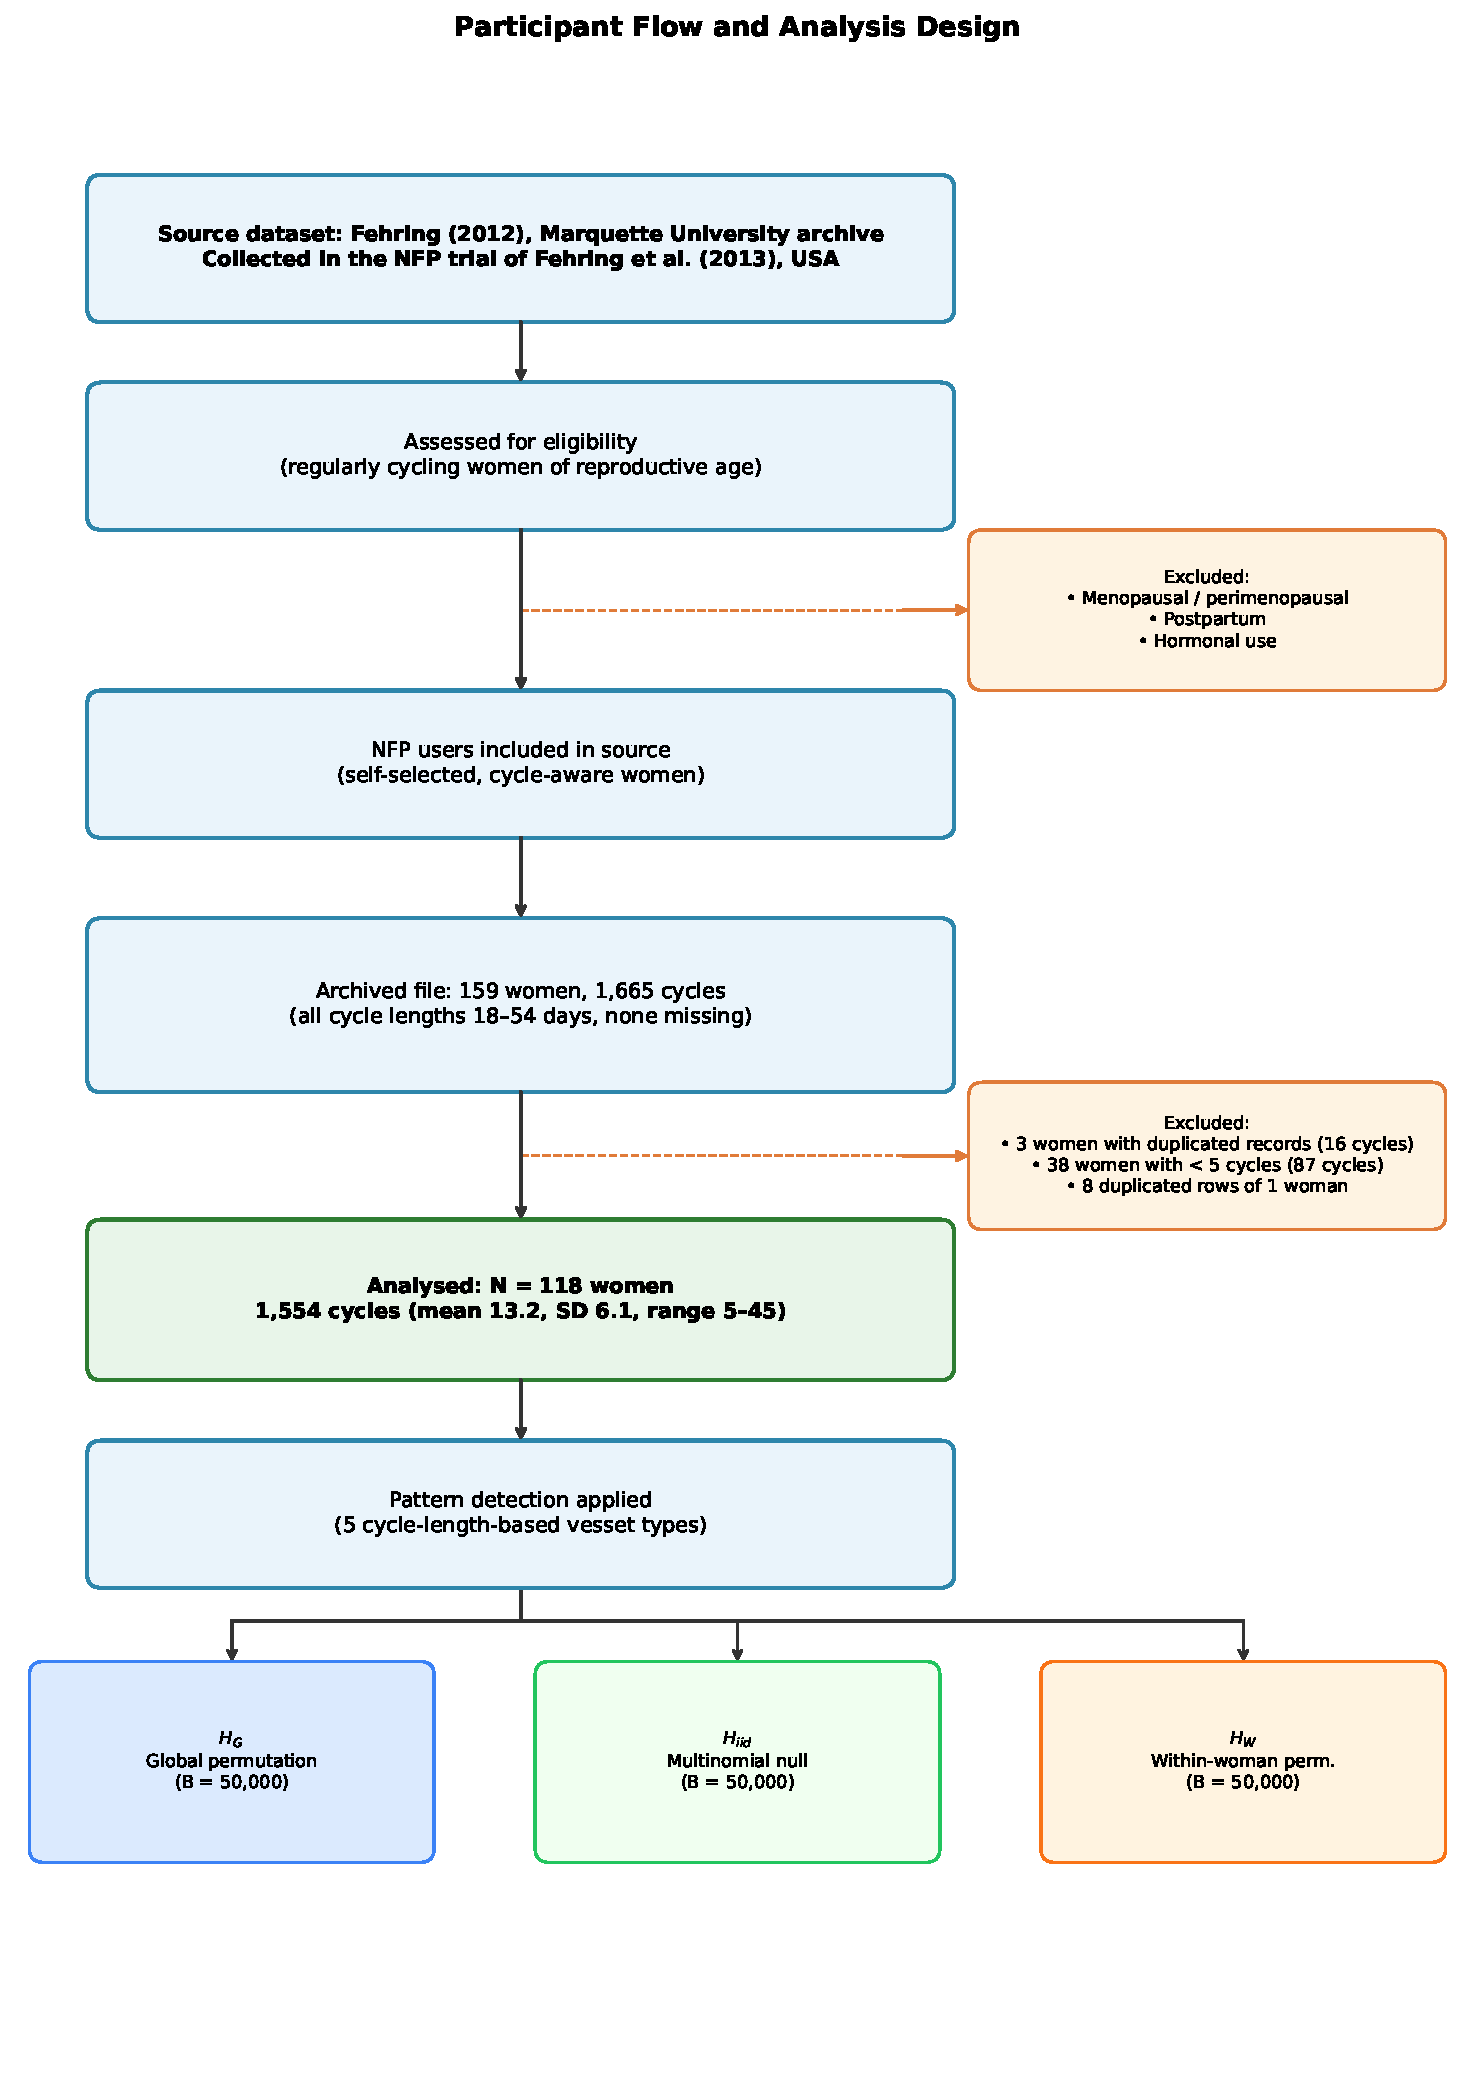
\includegraphics[width=0.75\textwidth]{fig2_consort_flow}
  \caption{Participant and data flow diagram. The source dataset
    (Fehring et al., 2013) comprises data from a multi-centre NFP cohort. After applying
    inclusion criteria (cycle length 18--54 days; complete cycle-length records), the
    analysed dataset comprised 118 women contributing 1,554 cycles. Five pattern types
    were detected per woman. Three complementary null models were then applied: $H_G$
    (global permutation, $N = 50{,}000$ iterations), $H_{iid}$ (multinomial null,
    $N = 50{,}000$ iterations), and $H_W$ (within-woman permutation null,
    $N = 50{,}000$ iterations per run).}
  \label{fig:consort}
\end{figure}

\subsection{Pattern Detection}

Pattern counting was performed within each woman's sequence independently; sequences
were never merged across women. Patient boundary pairs $(s_i, f_i)$ were encoded
explicitly and all counting loops were constrained to $[s_i, f_i]$. Extended runs of
the same pattern were counted as a single occurrence to avoid double-counting (e.g.,
four consecutive equal haflaga values constitute one Haflaga, not two). If a qualifying
run was interrupted by a discordant cycle and a new qualifying run of the same type
began later in the same woman's sequence, that resumed run was counted as a separate
event; the counts therefore reflect all distinct qualifying runs across each woman's
full history, not only the initial fixation event. All five functions
were validated against manually annotated examples and are available at
\url{https://[URL removed for peer review]}.

One counting implication follows directly from the definitions: Week-Dilug requires
$H_k = H_{k-1} = 30$ (two consecutive haflaga values equal to 30), whereas Haflaga-30
requires three consecutive haflaga values equal to 30. Therefore every Haflaga-30 sequence
automatically generates a Week-Dilug event in its first two cycles:
\[
  \{\text{Haflaga-30 sequence}\} \;\subseteq\; \{\text{Week-Dilug sequence}\}.
\]
This is set-theoretic inclusion, not merely statistical correlation, and it means
the Haflaga and Week-Dilug counts are not independent: the 3 Haflaga sequences with
$H = 30$ each contribute directly to the Week-Dilug count of 18.

\subsection{Null Models}
\label{sec:nullmodels}

Three null models address distinct scientific questions:
\begin{description}
  \item[$H_G$ \textnormal{(global exchangeability):}] All 1,554 cycle lengths exchangeable
    across women. Tests whether patterns exceed population-level chance.
  \item[$H_W$ \textnormal{(within-woman exchangeability):}] Each woman\'s cycles permuted uniformly at random within her own sequence (without replacement; observation indices are permuted, not unique values, so ties are handled correctly). Tests the null of \emph{within-woman exchangeability of the observed sequence}: whether temporal ordering creates excess patterns beyond what each woman's own cycle-length multiset predicts. This is not a general test of serial independence; a process with autocorrelation or latent trends could still fail to reject this null if those features do not produce additional exact vesset events.
  \item[$H_{iid}$ \textnormal{(multinomial i.i.d.):}] Each woman\'s cycles drawn i.i.d.
    from $\hat{F}$. Stronger than $H_G$: replaces observed values, not just ordering.
\end{description}

$H_G$ and $H_{iid}$ are the global nulls (permutation and multinomial respectively);
$H_W$ is the within-woman null. All three were run for $N = 50{,}000$ iterations (seed 17).
Table~\ref{tab:nullmodels} summarises the three null models side by side.

\begin{table}[H]
\centering
\caption{Comparison of the three null models. Each model preserves some aspects of the data
  structure while randomising others, encoding a distinct scientific question.}
\label{tab:nullmodels}
\small
\begin{tabular}{L{3.2cm} L{3.6cm} L{3.6cm} L{3.6cm}}
\toprule
& \textbf{$H_G$} (global perm.) & \textbf{$H_{iid}$} (multinomial) & \textbf{$H_W$} (within-woman) \\
\midrule
\textbf{Unit randomised} &
  Individual cycle records, pooled across all women &
  Pattern occurrence per cycle, drawn i.i.d.\ &
  Cycle order within each woman's own sequence \\[4pt]
\textbf{What is preserved} &
  Total cycle count; marginal haflaga distribution &
  Total count; observed marginal proportions &
  Each woman's multiset of cycle lengths and cycle count \\[4pt]
\textbf{What is destroyed} &
  Woman identity; within-woman ordering &
  All dependence; temporal structure &
  Within-woman temporal ordering only \\[4pt]
\textbf{Independence assumed} &
  None &
  Full i.i.d.\ (across time and women) &
  None (conditional permutation) \\[4pt]
\textbf{Scientific null} &
  Patterns arise from random assignment of cycles to women &
  Patterns arise from independent random events &
  Patterns arise from random ordering of each woman's own cycles \\[4pt]
\textbf{Implementation} &
  \texttt{np.random.permutation} on pooled haflaga values &
  Multinomial draw with observed proportions &
  Per-woman \texttt{np.random.permutation} (without replacement) \\
\bottomrule
\end{tabular}
\end{table}

\paragraph{Permutation test.}
At each iteration, the $n = 1{,}554$ haflaga values are randomly permuted without
replacement. This preserves the exact empirical marginal distribution and is
equivalent to assuming all $n!$ orderings are equally probable under $H_0$
\cite{edgington2007}.

\paragraph{Multinomial null.}
At each iteration, for each woman $i$ with $n_i$ cycles, a fresh sequence
$\tilde{H}_{i,1}, \ldots, \tilde{H}_{i,n_i} \overset{\text{i.i.d.}}{\sim} \hat{F}$
is drawn, where $\hat{F}$ is the empirical CDF of all 1,554 observed haflaga values.
This null directly encodes the hypothesis that cycles are \textit{independent} across
time within each woman \cite{anon2022phd}. It differs from a naive global bootstrap
(resampling with replacement from the pooled distribution, which is similar in spirit
to the multinomial null) in that each woman draws from the \emph{same} marginal $\hat{F}$,
ignoring between-woman heterogeneity in cycle-length distributions. The within-woman
permutation null ($H_W$) addresses this by conditioning each woman's simulated sequence
on her \emph{own} observed cycle-length multiset. A within-woman bootstrap (sampling
with replacement from each woman's own empirical distribution) was evaluated as an
alternative but rejected: because consecutive i.i.d.\ draws are independent whereas
permutation draws are negatively correlated (using a value reduces its availability at
the next position), the bootstrap inflates the expected count of repetition-based
patterns such as Haflaga --- from a null mean of 31.9 under permutation to 54.5 under
the bootstrap (a 71\% increase verified by $B = 50{,}000$ simulations). Permutation is
therefore preferred as the exact conditional randomisation test for the stated
exchangeability null; the bootstrap corresponds to a different iid-within-woman null,
and the two procedures are not directly comparable as more or less conservative in
general --- their different expected counts reflect the different scientific questions
they encode.

\subsection{Statistical Inference}
\label{sec:inference}

For each pattern $j$ and null model $m$ we computed: the observed count $O_j$; the
null mean $\bar{S}_j^{(m)}$ and SD $\sigma_j^{(m)}$; the z-score $z_j^{(m)} =
(O_j - \bar{S}_j^{(m)}) / \sigma_j^{(m)}$; and the two-sided empirical p-value
$p_j^{(m)} = 2\min\!\left(\tfrac{b_j^++1}{B+1},\,\tfrac{b_j^-+1}{B+1}\right)$,
where $b_j^+ = \#\{S_{j,r}^{(m)} \geq O_j\}$, $b_j^- = \#\{S_{j,r}^{(m)} \leq O_j\}$,
and $B = 50{,}000$, following the Monte Carlo convention of Davison \& Hinkley~\cite{davison1997}.
All marginal tests use two-sided p-values; the direction and magnitude of departure
from the null are separately reported via $z$-scores. The joint Mahalanobis distance
is inherently two-sided --- it measures displacement from the null centre in any
direction --- and serves as an omnibus test of whether the observed count vector is
jointly unusual.

The \textbf{joint multivariate test} uses the \textbf{Mahalanobis distance} as the test statistic:
\begin{equation}
  D_M^{(m)} = \sqrt{\bigl(\mathbf{O}-\boldsymbol{\mu}^{(m)}\bigr)^\top
               \bigl(\hat{\Sigma}^{(m)}\bigr)^{-1}
               \bigl(\mathbf{O}-\boldsymbol{\mu}^{(m)}\bigr)},
  \label{eq:mahalanobis}
\end{equation}
with p-value equal to the fraction of null replicates where the simulated $D_M$ exceeded
the observed value. Unlike Bonferroni--Holm correction --- which, while valid under arbitrary
dependence, is conservative when tests are positively correlated --- this joint permutation test operates on the full count vector simultaneously,
respecting the dependence structure. Note that this is a single global test of
the multivariate null, not an FWER procedure across the five component tests.
The joint Mahalanobis test is the \textbf{primary multivariate inferential procedure};
the individual Holm-corrected marginal tests are reported as \textbf{secondary descriptive summaries}
of pattern-specific effect sizes and should not be used in place of the joint test
for global inference. Conceptually related quadratic-form permutation tests exist
(e.g., energy-distance statistics; \citealp{king2018}) --- the contribution here is
an adaptation of this framework to dependent, sequentially-defined count vectors
in longitudinal cycle data; to our knowledge this specific application is new. Mahalanobis distance correctly standardises each component by its null variance and accounts for inter-component correlations. Non-diagonal terms in $\hat{\Sigma}$ are expected a priori: the set-theoretic containment of Haflaga-30 within Week-Dilug and the polynomial proximity of Dilug-in-Dilug to Haflaga (Section~\ref{sec:mathdep}) imply that the five pattern counts are not marginally independent, so a diagonal standardisation would misrepresent the dependence structure. $\hat{\Sigma}^{(m)}$ is estimated empirically from the $B = 50{,}000$ simulated count vectors under each null model: $\hat{\Sigma}^{(m)} = \frac{1}{B-1}\sum_{r=1}^{B}(\mathbf{S}^{(m,r)} - \bar{\mathbf{S}}^{(m)})(\mathbf{S}^{(m,r)} - \bar{\mathbf{S}}^{(m)})^\top$, where $\mathbf{S}^{(m,r)}$ is the count vector from replicate $r$ and $\bar{\mathbf{S}}^{(m)}$ is the Monte Carlo mean; this is the sample covariance of the null replicates, not the sample covariance of the observations. The result is a $5 \times 5$ matrix. Condition numbers of 4.4 (permutation null) and 5.4 (multinomial null) confirm that the matrix is well-conditioned and the inversion is numerically stable; note that a low condition number establishes numerical stability of the inversion, not that Mahalanobis distance is the most powerful statistic for every scientific alternative (the statistic detects significant departure in any direction, not specifically the positive direction; the direction of displacement is separately reported via the individual $z$-scores). The Euclidean displacement $D_E^{(m)} = \|\mathbf{O} - \boldsymbol{\mu}^{(m)}\|_2$ is shown geometrically in the figures as the length of the dashed displacement line.

The \textbf{primary joint test} applies Eq.~\ref{eq:mahalanobis} to all five patterns simultaneously, using the full $5\times5$ empirical null covariance $\hat{\Sigma}$ (condition numbers 4.4--5.4; well-conditioned). The null hypothesis $H_0^{(5)}$ states that the observed 5-pattern count vector follows the joint null distribution under $H_W$ (or $H_G$ / $H_{iid}$); the alternative $H_1^{(5)}$ is that the observed vector is displaced from the null centre in any direction.

An \textbf{exploratory focused analysis} restricts the joint test to the three structurally dependent patterns --- Haflaga, Week-Dilug, and Dilug-in-Dilug --- to visualise the displacement geometry in three dimensions (Figure~\ref{fig:joint3panels}). This subspace is motivated by algebraic structure established prior to data inspection:
\begin{itemize}
  \item Haflaga-30 $\subseteq$ Week-Dilug by set-theoretic containment
    (Section~\ref{sec:mathdep}), creating a deterministic co-occurrence dependency.
  \item Dilug-in-Dilug is the degree-2 polynomial neighbour of degree-0 Haflaga,
    creating algebraic proximity.
\end{itemize}
This analysis is designated exploratory because the structural motivation does not constitute a pre-registered exclusion of Dilug and Week; the primary inference uses all five patterns.

\paragraph{Sensitivity.}
The joint test is sensitive primarily to the Haflaga component, which contributes
the largest standardised excess ($z = 4.51$) and --- after variance standardisation
by the Mahalanobis metric --- the largest weight. Under the global permutation null,
the observed $D_M = 5.10$ exceeds the 99.9th percentile of the null distribution.

Pairwise \textbf{Spearman rank correlations} were computed between per-woman
pattern rates (number of pattern events divided by number of cycles). Using rates
rather than binary indicators mitigates the cycle-count exposure confound: women
with more cycles have more opportunities to satisfy any pattern, and normalising
by cycle count reduces but does not eliminate this exposure difference (the permutation
randomises the rate vector rather than conditioning on cycle count). Two-sided permutation $p$-values
(50,000 permutations of one variable's rate vector) with Holm--Bonferroni correction
across the 10 pairs were used for inference. $\alpha = .05$ throughout.

\paragraph{Simulation pipeline.}
Algorithm~\ref{alg:sim} provides a formal pseudocode description of the full
simulation pipeline for reproducibility.

\paragraph{Minimum run-length examples.}
To clarify the counting convention, consider a single woman's haflaga sequence.
A run of length 2: $(29, 29)$ qualifies as Week-Dilug (if $H = 30$) or Week but
\emph{not} as Haflaga (which requires at least 3). A run of length 3: $(28, 28, 28)$
qualifies as Haflaga (and as Week if 28 $\in \mathcal{W}$). A run of length 4:
$(27, 29, 31, 33)$ qualifies as Dilug ($d = +2$, constant first difference, $\geq 3$ cycles)
but also as Dilug-in-Dilug only if a second constant non-zero difference exists ---
this sequence has second differences $(2-2, 2-2) = (0, 0)$, so it does \emph{not}
qualify as Dilug-in-Dilug (which requires $d \neq 0$ in the second differences).
Instead $(27, 28, 30, 33)$ has first differences $(1, 2, 3)$ and second differences
$(1, 1)$, giving $d = 1 \neq 0$, so it qualifies as Dilug-in-Dilug (minimum 4 cycles).

\begin{algorithm}[H]
\caption{Full simulation pipeline}
\label{alg:sim}
\begin{algorithmic}[1]
\Require Dataset $\mathcal{D} = \{(H_{i,1},\ldots,H_{i,n_i})\}_{i=1}^{N}$ ($N$ women),
         patterns $j = 1,\ldots,5$, iterations $B$, seed
\State Compute observed counts $\mathbf{O} = (O_1,\ldots,O_5)$ via pattern detection
\For{$r = 1$ to $B$}
  \State // Global permutation null ($H_G$): shuffle all $\sum_i n_i$ haflaga values
  \State $\mathbf{H}^{(G)} \leftarrow \operatorname{Permute}(\bigcup_i \{H_{i,k}\})$;
         re-assign to women preserving $n_i$
  \State $\mathbf{S}^{(G,r)} \leftarrow \operatorname{Count}(\mathbf{H}^{(G)})$
  \State // Multinomial null ($H_{iid}$): draw each $H_{i,k}$ iid from marginal distribution
  \State $\mathbf{H}^{(M)} \leftarrow \operatorname{Multinomial}(p_1,\ldots,p_K; \text{total } \textstyle\sum_i n_i)$
  \State $\mathbf{S}^{(M,r)} \leftarrow \operatorname{Count}(\mathbf{H}^{(M)})$
  \State // Within-woman permutation null ($H_W$): shuffle within each woman
  \For{$i = 1$ to $N$}
    \State $\mathbf{H}^{(W)}_i \leftarrow \operatorname{Permute}(H_{i,1},\ldots,H_{i,n_i})$
           \Comment{without replacement}
  \EndFor
  \State $\mathbf{S}^{(W,r)} \leftarrow \operatorname{Count}(\mathbf{H}^{(W)})$
\EndFor
\State Estimate $\hat{\Sigma}^{(m)} \leftarrow \operatorname{SampleCov}(\{\mathbf{S}^{(m,r)}\}_{r=1}^{B})$
       for each $m \in \{G, M, W\}$
\For{$m \in \{G, M, W\}$}
  \State Null mean $\boldsymbol{\mu}^{(m)} \leftarrow B^{-1}\sum_r \mathbf{S}^{(m,r)}$
  \State Mahalanobis statistic:
         $D_M^{(m)} \leftarrow \sqrt{(\mathbf{O}-\boldsymbol{\mu}^{(m)})^\top
         (\hat{\Sigma}^{(m)})^{-1}(\mathbf{O}-\boldsymbol{\mu}^{(m)})}$
  \State $p_j^{(m)} \leftarrow (|\{r : S_j^{(m,r)} \geq O_j\}|+1)/(B+1)$
         for each pattern $j$ \Comment{two-sided}
  \State $p_{D_M}^{(m)} \leftarrow (|\{r : D_M^{(m,r)} \geq D_M^{(m)}\}|+1)/(B+1)$
\EndFor
\end{algorithmic}
\end{algorithm}

% ─── 4. Results ───────────────────────────────────────────────────────────────
\section{Results}

\subsection{Per-Pattern Hypothesis Tests}

Observed counts were: Haflaga $= 26$, Dilug $= 61$, Week $= 32$, Week-Dilug $= 18$,
Dilug-in-Dilug $= 27$. Of the 26 Haflaga sequences, 3 had value $H = 30$, each
automatically constituting a Week-Dilug event (set-theoretic inclusion); of the 27
Dilug-in-Dilug sequences, 16 had second difference $|d| = 1$ (near-Haflaga).
Table~\ref{tab:results} presents the full results under both null models.
Figures~\ref{fig:nulldists} and \ref{fig:zscores} display the null distributions and
effect sizes.

\begin{table}[H]
\centering
\caption{Permutation and multinomial null-model results ($N = 50{,}000$ iterations).
  \textit{Null Mean} and \textit{Null SD} are from the permutation null. Bold
  $p$-values are significant at $\alpha = .05$ (two-sided).}
\label{tab:results}
\smallskip
\begin{tabular}{L{3.0cm} C{1.2cm} C{1.6cm} C{1.4cm} C{1.4cm} C{1.6cm} C{1.6cm}}
\toprule
\textbf{Pattern} & \textbf{Obs.} & \textbf{Null Mean}
  & \textbf{Null SD} & \textbf{$z$}
  & \textbf{Perm.~$p$} & \textbf{Multi.~$p$} \\
\midrule
Haflaga         & 26 & 11.30 & 3.26 & $+4.51$ & $\mathbf{<.001}$ & $\mathbf{<.001}$ \\
Dilug           & 61 & 48.93 & 6.60 & $+1.83$ & $.087$           & $.086$           \\
Week            & 32 & 27.00 & 4.03 & $+1.24$ & $.133$           & $.188$           \\
Week-Dilug      & 18 & 16.27 & 3.28 & $+0.53$ & $.345$           & $.366$           \\
Dilug-in-Dilug  & 27 & 27.17 & 5.04 & $-0.03$ & $.543$           & $.544$           \\
\bottomrule
\end{tabular}
\end{table}

\begin{figure}[H]
  \centering
  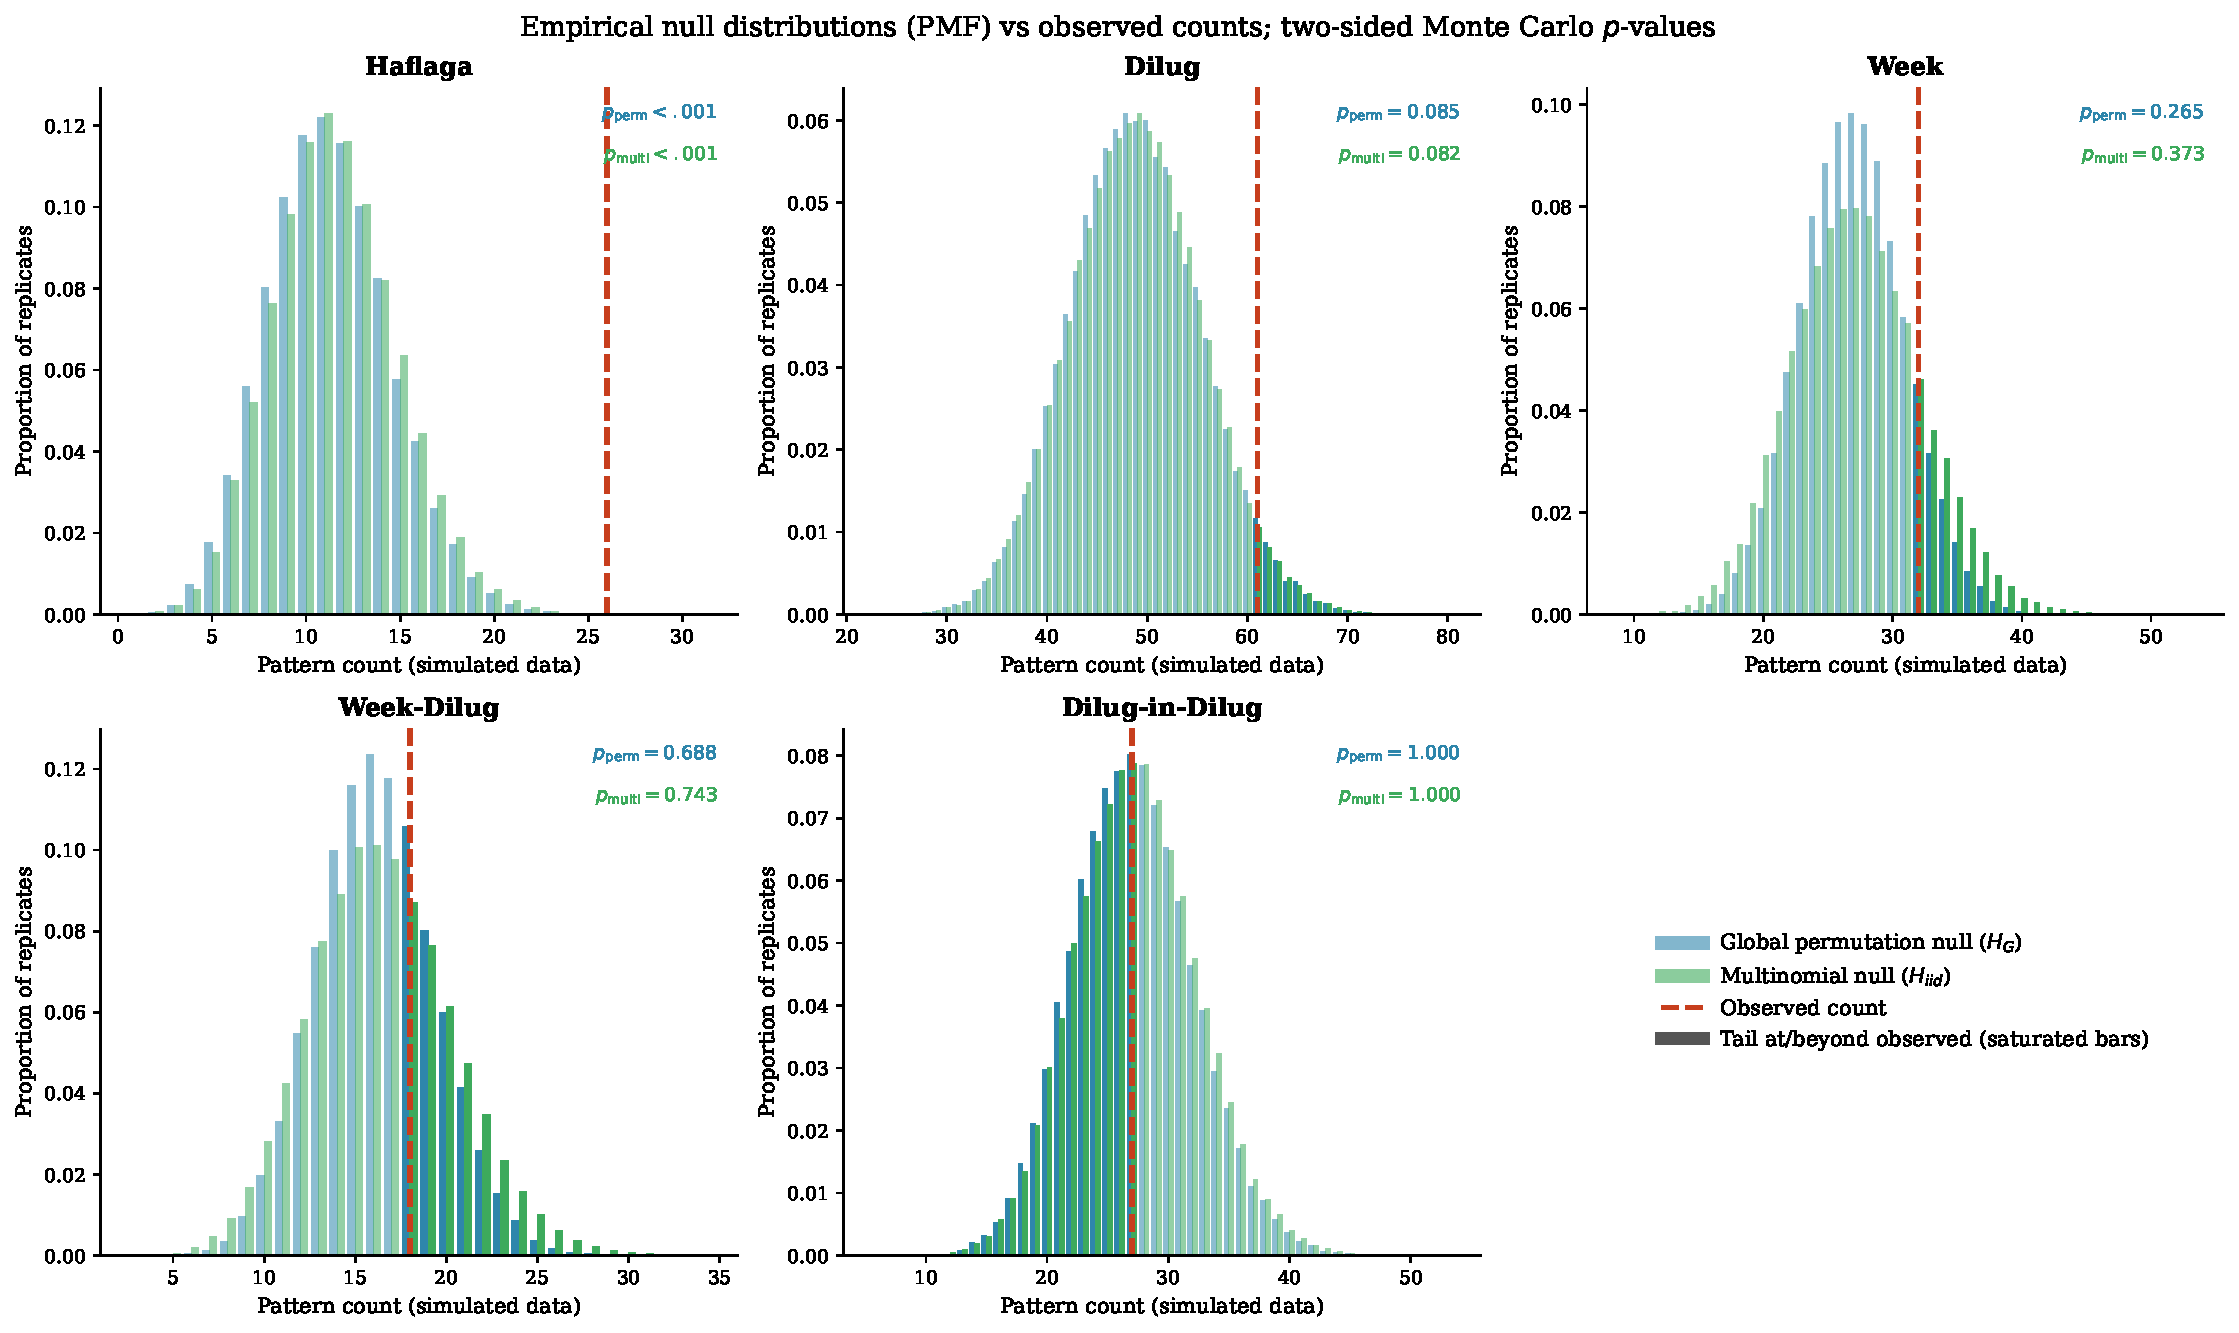
\includegraphics[width=\textwidth]{fig3_null_distributions}
  \caption{Empirical null distributions (shown as smoothed density estimates) vs.\ observed counts for each vesset pattern
    under the permutation (solid curve) and multinomial (dashed curve) null models.
    The underlying null distributions are discrete; the smoothed curves are shown for
    visual comparison only, with the primary inference based on the empirical PMF (fraction
    of $B = 50{,}000$ simulations meeting or exceeding the observed count).
    The vertical dotted line marks the observed count; the shaded region is the
    two-sided p-value area. Haflaga shows a clearly right-displaced observed
    value; Dilug-in-Dilug falls on its null mean.}
  \label{fig:nulldists}
\end{figure}

\begin{figure}[H]
  \centering
  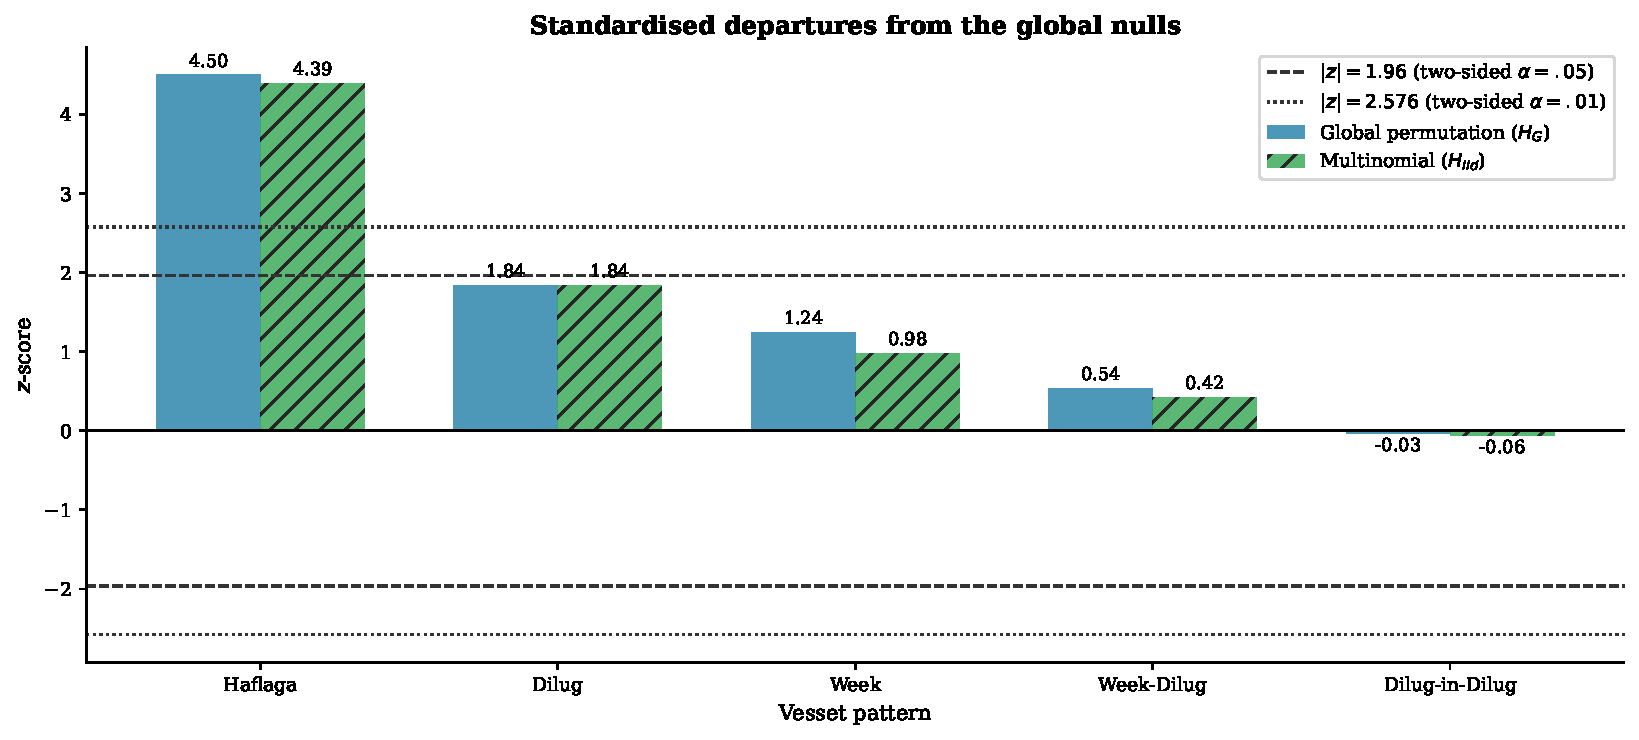
\includegraphics[width=0.88\textwidth]{fig4_zscores}
  \caption{Effect sizes ($z$-scores) under permutation (solid bars) and multinomial (hatched bars)
    null models. Dashed and dotted lines mark two-sided $\alpha = .05$ ($|z| = 1.96$) and
    $\alpha = .01$ ($|z| = 2.576$) thresholds (two-sided tests; see Table~\ref{tab:results}).
    $z$-scores differ between nulls (e.g., Week: 1.24 vs.\ 0.98) because each null has its own mean and SD.
    Only Haflaga exceeds the $\alpha = .05$ threshold; both null models are in close agreement.}
  \label{fig:zscores}
\end{figure}

Haflaga showed the strongest effect: 26 occurrences vs.\ a null mean of 11.30, more
than 4.5 standard deviations above chance ($z = 4.51$, exact Monte Carlo $p = 3/50{,}001 \approx .00006$). Crucially, under
the permutation null only \textbf{2 of 50,000} simulations reached or exceeded 26 ---
the observed count ties the simulation maximum. Applying Holm--Bonferroni correction
across the five pattern tests, only Haflaga remains significant after FWER control
(Holm-adjusted $p = .0003$). Dilug is not significant ($p = .087$, Holm-adjusted $p = .346$) and should be regarded
as an exploratory finding requiring replication. Week, Week-Dilug, and Dilug-in-Dilug are not significant.
These marginal results are complementary summaries; the primary multivariate inference is
the joint Mahalanobis test (Section~\ref{sec:joint}), which operates on the full count
vector simultaneously without multiple-comparison correction.

\subsection{Agreement Between Null Models}

The permutation and multinomial null models are in close agreement across all five
patterns (maximum difference in p-values: 0.055). Figure~\ref{fig:cdfs} shows the
empirical CDFs, confirming the two nulls produce nearly identical distributions for
each pattern. The close agreement is a numerical observation; whether and under what
conditions the two procedures converge asymptotically depends on the specific sampling
model and is not formally established here.

\begin{figure}[H]
  \centering
  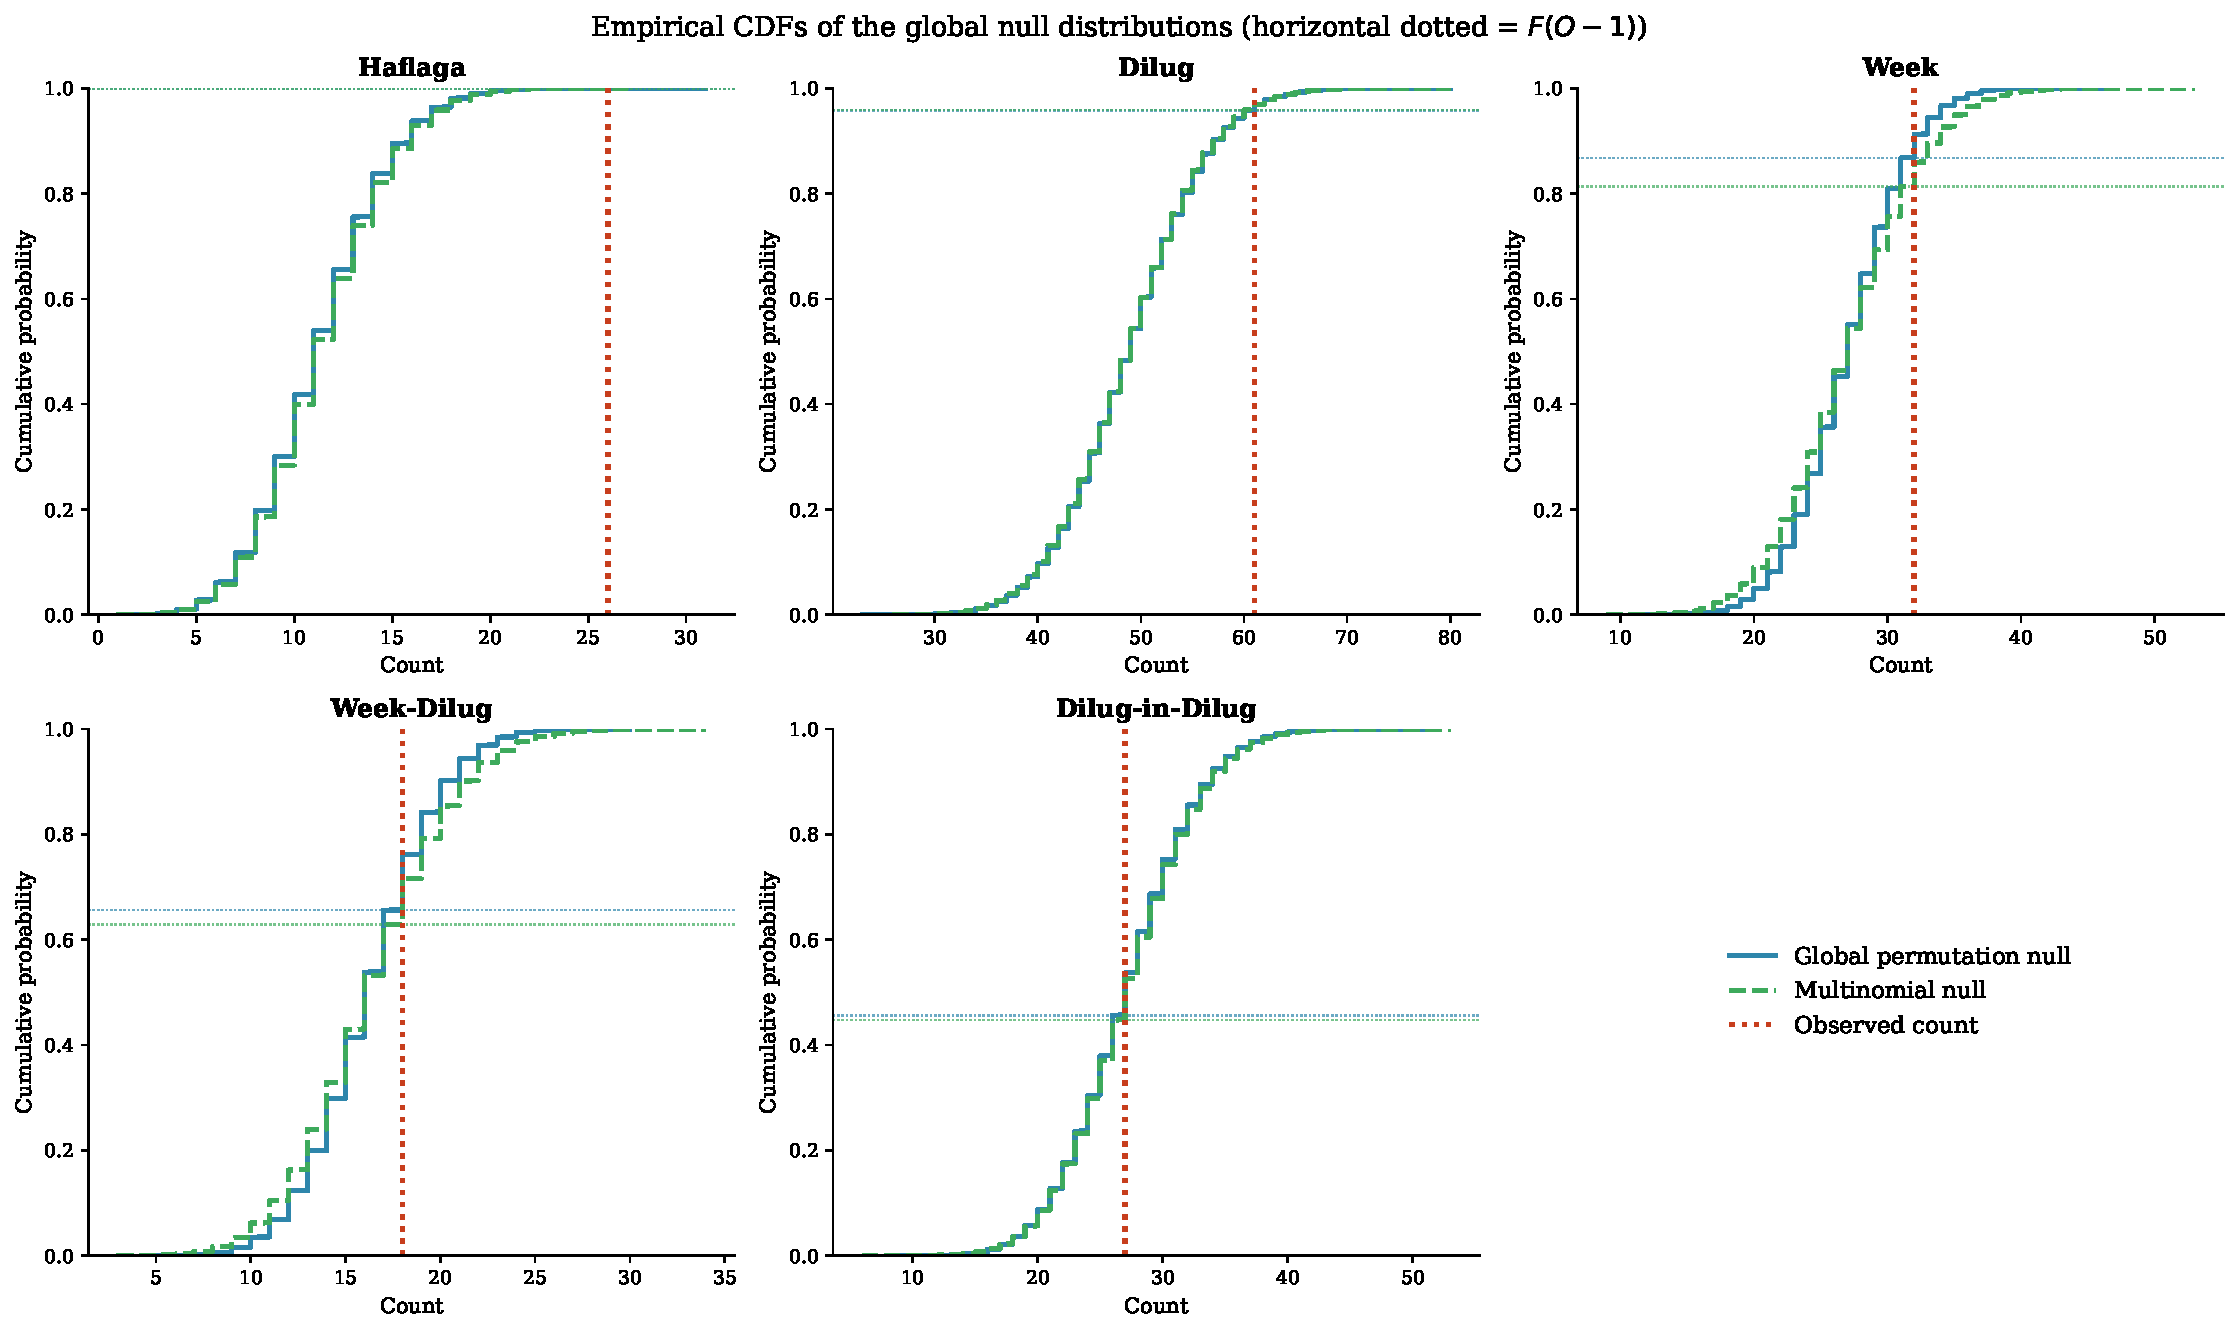
\includegraphics[width=\textwidth]{fig5_cdfs}
  \caption{Empirical CDFs of null distributions for each pattern under permutation
    (solid curve) and multinomial (dashed curve) nulls. The vertical dotted line
    marks the observed count; horizontal dotted lines indicate $1-p$. The close
    overlap confirms robustness to the choice of null model.}
  \label{fig:cdfs}
\end{figure}


\subsection{Within-Woman Permutation Analysis}
\label{sec:stratified}

The global permutation and multinomial null models permute or resample haflaga values
\emph{across} all 118 women, thereby removing between-woman heterogeneity in cycle
regularity. As noted in Section~\ref{sec:nullmodels}, this means both global nulls
test whether vesset patterns are more frequent than expected if all women drew from
the same population distribution --- not whether patterns are more frequent than
expected \emph{given each woman's own level of regularity}. These are distinct
scientific questions.

To address the within-woman question, we implemented a \textbf{within-woman permutation} null ($H_W$): for each woman independently, her cycle-length sequence is randomly permuted (shuffled without replacement), preserving her individual cycle-length \emph{multiset} while randomising the temporal ordering. This null encodes the hypothesis that the
\emph{temporal ordering} of cycles within a woman does not create patterns beyond what her
own cycle-length values (taken in random order) would predict. The null is specifically
a conditional exchangeability null: it does not test general serial independence, and a
process with autocorrelation or trend structure could still fail to reject it if such
structure does not translate into additional exact vesset-pattern occurrences.

\paragraph{Implementation.}
For each of the 118 women independently, her cycle-length sequence is permuted uniformly at random (without replacement). All women are included with no exclusion threshold. The aggregate null is generated by summing the permuted count vectors across all 118 women, producing $B = 50{,}000$ realisations of the joint count vector.

\paragraph{Results.}
Table~\ref{tab:stratified} presents the results. Under the within-woman null,
\emph{no pattern is individually significant}. All five observed counts fall
\emph{below} their within-woman null means (all $z < 0$). Dilug-in-Dilug has the most extreme z-score ($z = -2.07$, two-sided $p = .040$, Holm-corrected $p = .198$); this does not survive multiple-comparison control and should be regarded as exploratory. The negative direction --- the observed count (27) is well below the within-woman null mean (39.1) --- indicates that real temporal ordering of cycles produces fewer DiD events than random shuffling of the same cycle lengths would predict, which is consistent with DiD detecting genuine second-order cycle regularity rather than chance co-occurrence of lengths.
The joint test is also non-significant: Mahalanobis $D_M = 2.95$ ($p = .121$).
Tables~\ref{tab:stratified} and~\ref{tab:power} both use the primary 50,000-run
simulation (seed 17) to ensure full numerical consistency of $\mu_W$, $\sigma_W$,
and $z_{\text{obs}}$ across all results.

\begin{table}[H]
\centering
\caption{Within-woman permutation null ($H_W$) results ($N = 50{,}000$; all $n = 118$ women; each woman's sequence permuted uniformly at random without replacement). All observed counts fall below their within-woman null means. $p$-values are two-sided: $2\min\!\bigl((b^++1)/(B+1),\,(b^-+1)/(B+1)\bigr)$.}
\label{tab:stratified}
\smallskip
\begin{tabular}{L{3.2cm} C{1.2cm} C{1.6cm} C{1.4cm} C{1.4cm} C{1.6cm}}
\toprule
\textbf{Pattern} & \textbf{Obs.} & \textbf{Null Mean} & \textbf{Null SD}
  & \textbf{$z$} & \textbf{$p$} \\
\midrule
Haflaga         & 26 & 31.85 & 4.68 & $-1.25$ & $.249$ \\
Dilug           & 61 & 67.07 & 7.36 & $-0.83$ & $.455$ \\
Week            & 32 & 33.81 & 3.88 & $-0.47$ & $.741$ \\
Week-Dilug      & 18 & 20.94 & 3.22 & $-0.91$ & $.454$ \\
Dilug-in-Dilug  & 27 & 39.14 & 5.86 & $-2.07$ & $.040$ \\
\midrule
\multicolumn{6}{l}{Joint: $D_M = 2.95$ ($p = .121$)} \\
\bottomrule
\end{tabular}
\end{table}

Figure~\ref{fig:stratified} illustrates the contrast between the global and
within-woman nulls for each pattern. The shift in the null distribution is striking:
for Haflaga, the global null is centred around 10, while the within-woman null is
centred around 27 --- far above the observed count of 26 (all 118 women).

\begin{figure}[H]
  \centering
  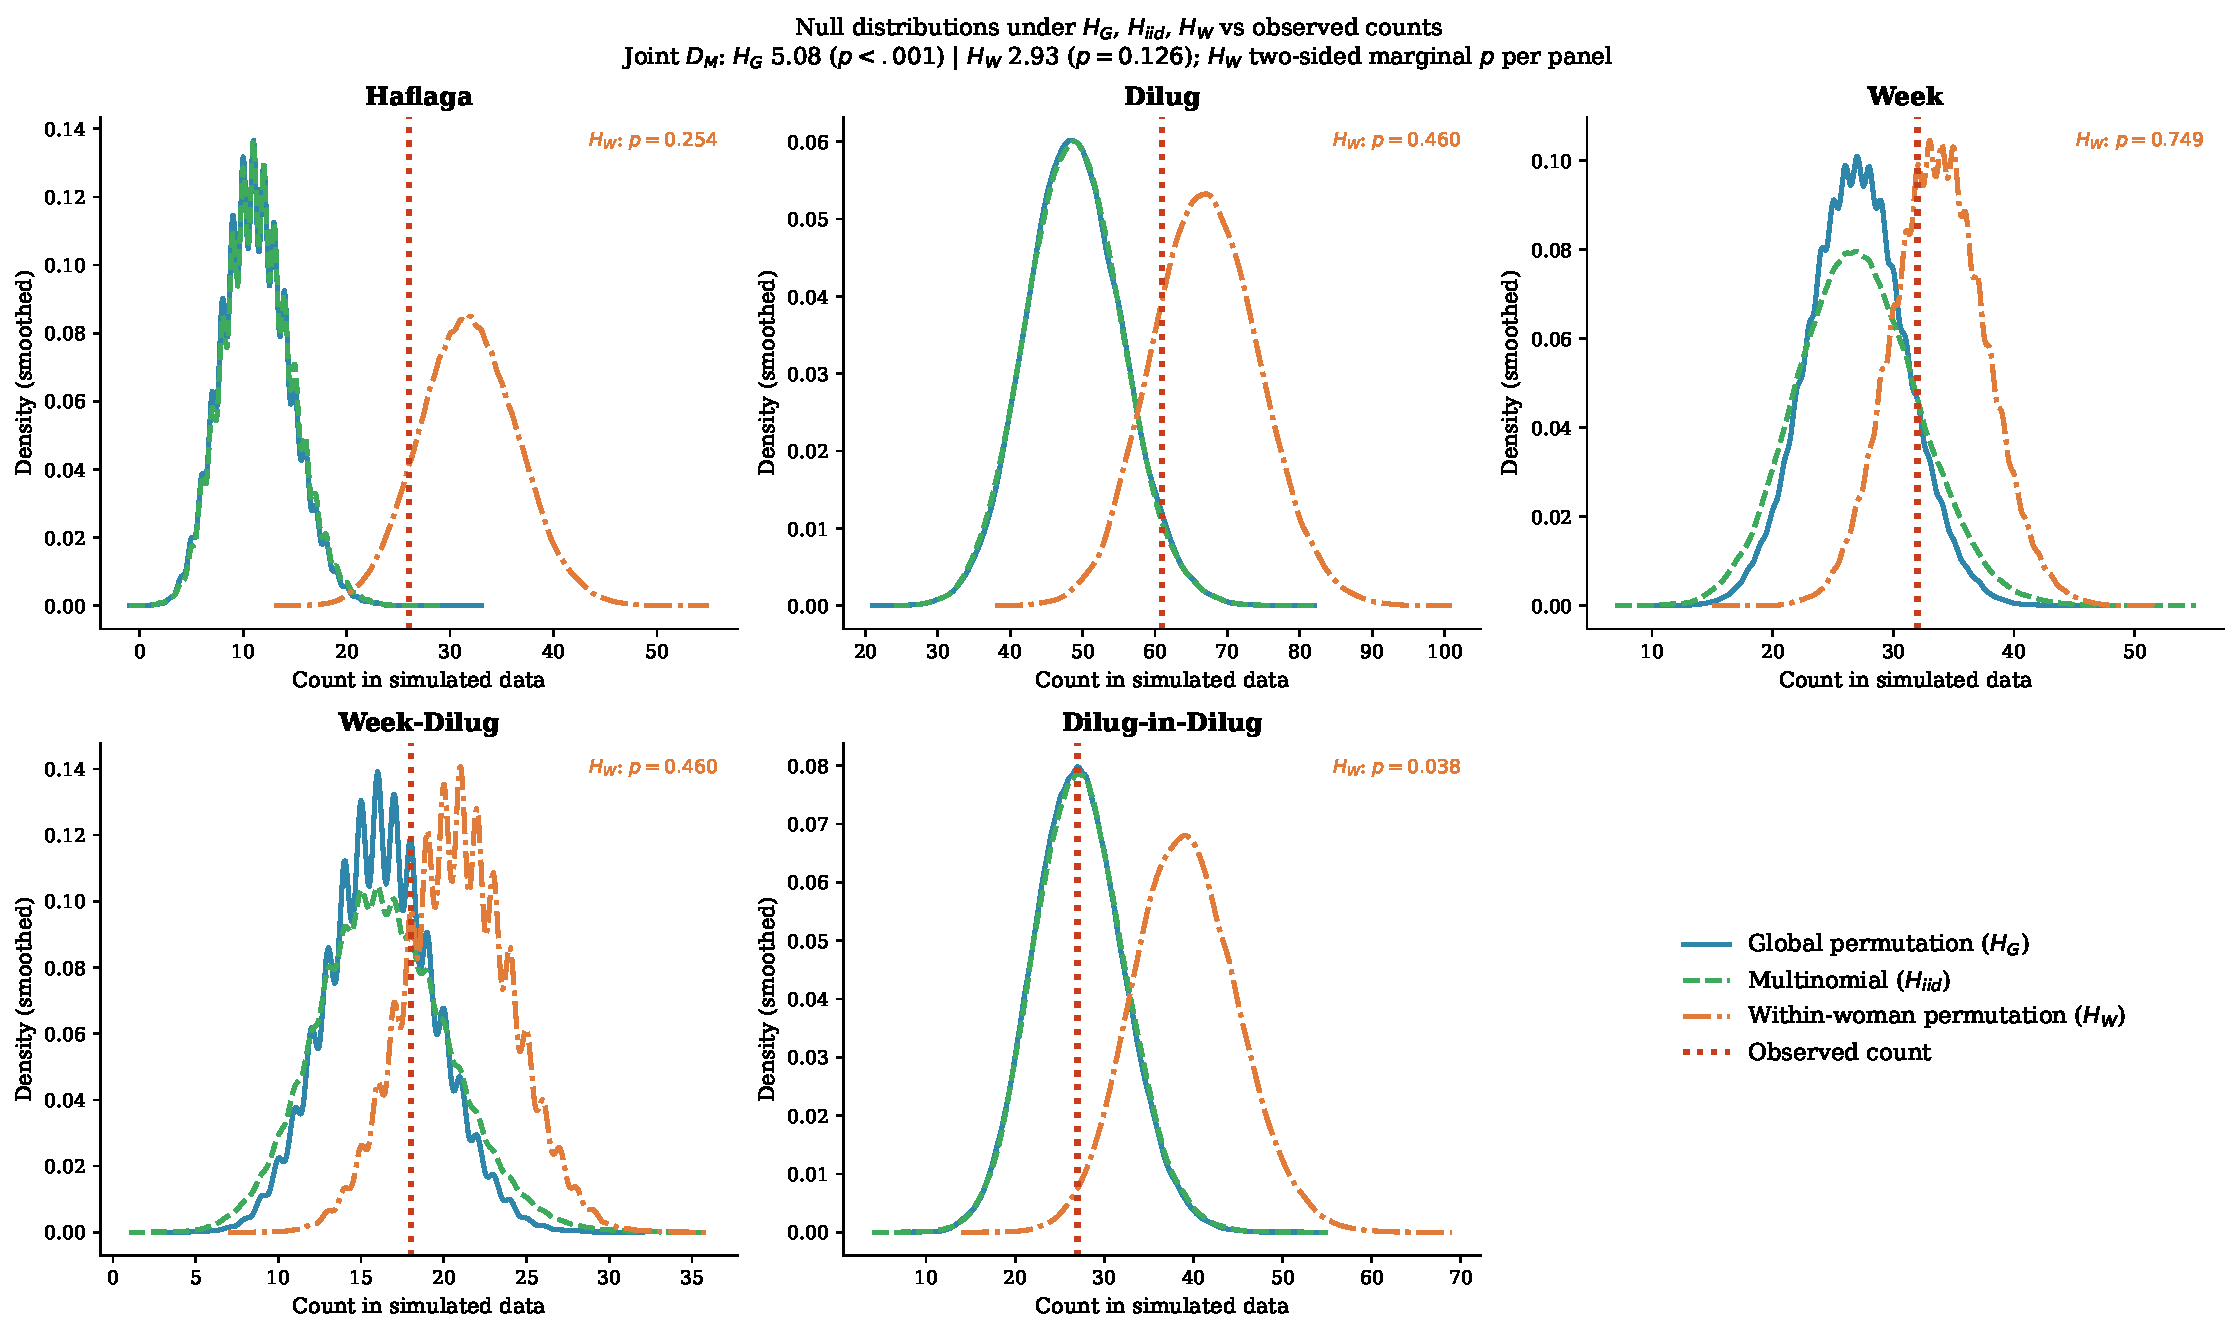
\includegraphics[width=\textwidth]{fig6_stratified_comparison}
  \caption{Null distributions ($H_G$, $H_{iid}$, $H_W$) for each pattern under three null models:
    global permutation (light fill), global multinomial (medium fill),
    and within-woman permutation (dark fill), all $N = 118$ women.
    Dashed vertical line: observed count. The joint panel shows Mahalanobis $D_M$
    histograms; both global nulls are highly significant ($p < .001$)
    while the within-woman null is non-significant ($D_M = 2.95$, $p = .121$).}
  \label{fig:stratified}
\end{figure}

\paragraph{Interpretation.}
The two nulls answer different scientific questions and are both valid:
\begin{itemize}
  \item The \textbf{global null} tests: \emph{are vesset patterns more frequent than
    expected if all cycle lengths were exchangeable across all women?} The answer is
    yes for Haflaga ($p < .001$ after Holm correction), reflecting that vesset patterns
    are concentrated among women who are intrinsically more regular.
  \item The \textbf{within-woman null} tests: \emph{given each woman's own level of
    cycle regularity, are the temporal arrangements unusually structured?} The answer
    is no --- under the within-woman exchangeability null, this dataset provides
    no detectable evidence that temporal ordering adds structure beyond each
    woman's own cycle-length distribution.
\end{itemize}
Together, these results suggest that halachic vesset rules --- particularly Haflaga
--- constitute an empirical codification of individual menstrual regularity: the rules
correctly identify the subset of women whose cycles are intrinsically stable, and
formalise that stability as an anticipatory pattern. Whether this reflects deliberate
halachic wisdom or fortuitous alignment with biology is beyond the scope of the
present analysis. A companion study examining the practical forecasting efficiency of halachic
vesset rules --- how accurately they predict the next menstruation onset, and at what cost in unnecessary abstinence days --- is in preparation \cite{anon_planned}.

\subsection{Joint Multivariate Test}
\label{sec:joint}

\paragraph{Primary test: 5-pattern Mahalanobis.}
The primary joint test applies to all five patterns simultaneously (Section~\ref{sec:inference}).
Under the global permutation null, $D_M = 5.10$ ($p < .001$; 0 of 50,000 null replicates
exceeded the observed $D_M$); under the multinomial null, $D_M = 4.84$ ($p < .001$; 0 of 50,000).
Under the within-woman null --- the primary scientific test --- $D_M = 2.95$ ($p = .121$;
6,037 of 50,000 null replicates exceeded the observed $D_M$), confirming non-detection of
excess patterning under within-woman exchangeability.
Figure~\ref{fig:joint1d} shows the 5-pattern Mahalanobis null distributions for all three null models.

\paragraph{Exploratory: focused 3-pattern subspace.}
An exploratory analysis restricts the joint test to the three structurally dependent
patterns (Haflaga, Week-Dilug, Dilug-in-Dilug; see Section~\ref{sec:inference}).
Under the global permutation null, $D_M = 4.52$ ($p < .001$); under the multinomial null,
$D_M = 4.36$ ($p < .001$); under the within-woman null, $D_M = 2.68$ ($p = .066$).
Figure~\ref{fig:joint3panels} illustrates the displacement geometry in this 3-pattern subspace.
Results are consistent with the primary 5-pattern analysis; the slight difference
($D_M^{H_W} = 2.68$ vs.\ $2.95$) reflects exclusion of Dilug and Week from the subspace.

\begin{figure}[H]
  \centering
  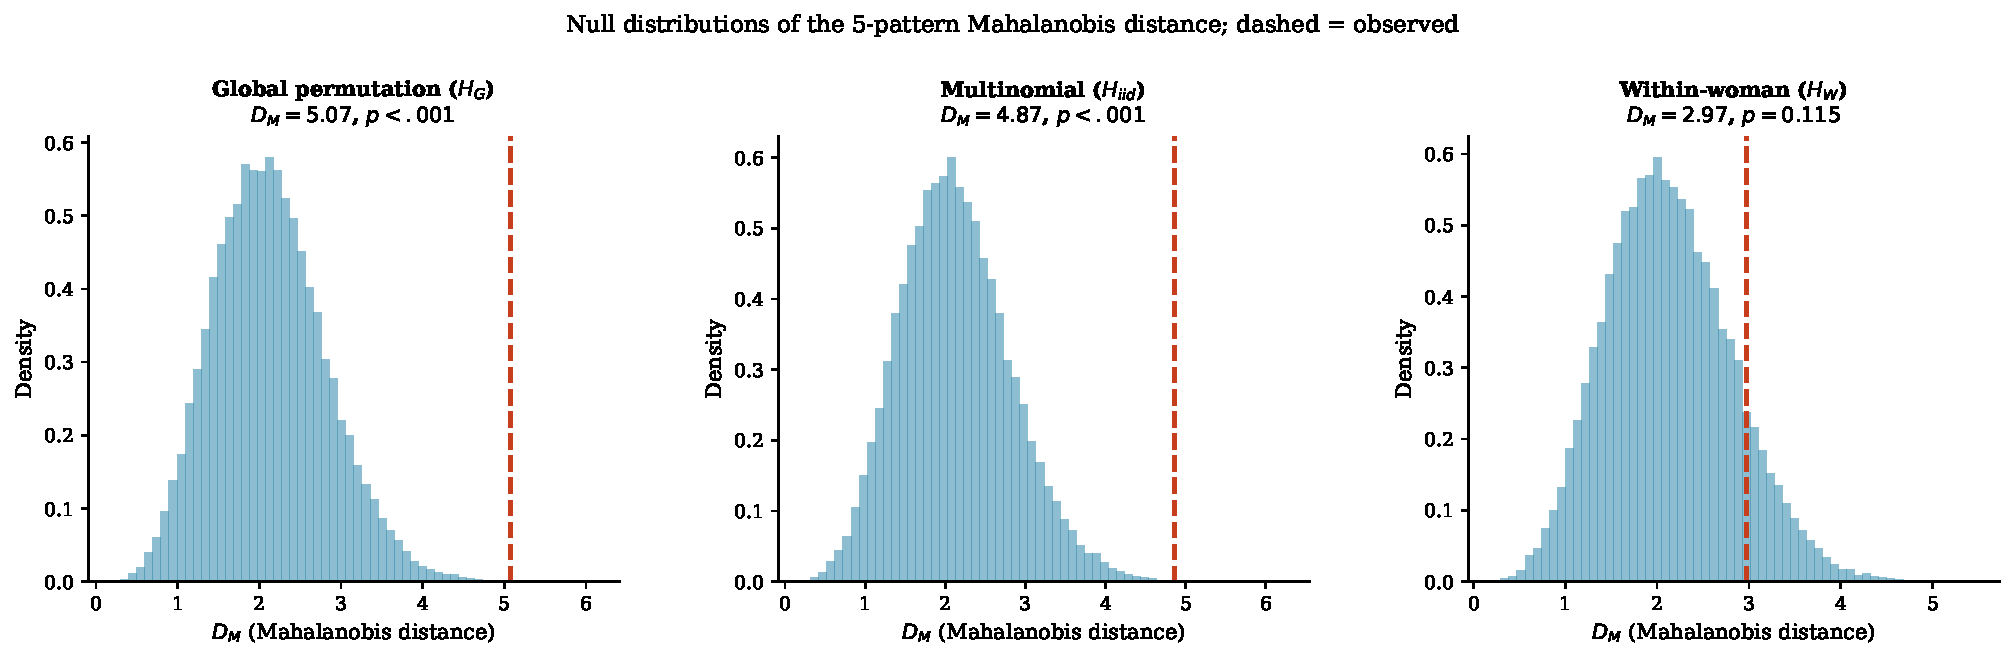
\includegraphics[width=\textwidth]{fig7_dm_nulldist}
  \caption{Robustness check: null distributions of the 5-pattern Mahalanobis distance
    $D_M$ (Eq.~\ref{eq:mahalanobis}) under the permutation ($H_G$, left),
    multinomial ($H_{iid}$, centre), and within-woman ($H_W$, right) nulls.
    The dashed line marks the observed $D_M$; the shaded region is the upper-tail
    area corresponding to the empirical p-value.
    Under $H_G$ and $H_{iid}$ the observed vector lies far in the tail ($p < .001$);
    under $H_W$ the displacement is non-significant ($D_M = 2.95$, $p = .121$).}
  \label{fig:joint1d}
\end{figure}

\subsection{Pairwise Dependence Tests and Focused Joint Test}
\label{sec:chisq}

The structural relationships of Section~\ref{sec:mathdep} motivate a prior prediction
for the pairwise dependence tests, but the two predicted pairs have different logical
status and should be interpreted accordingly.

\textbf{Layer 1 — Deterministic logical structure.} Haflaga-30 is a subset of
Week-Dilug by definition: any woman who establishes a Haflaga sequence at $H = 30$
necessarily satisfies the Week-Dilug criterion. This is a logical implication of the
pattern definitions, not an empirical finding.

\textbf{Layer 2 — Exploratory empirical associations.} Haflaga $\times$
Dilug-in-Dilug rests on the algebraic proximity argument (Section above): a DiD
sequence with $|d| = 1$ is close to a constant, so co-occurrence with Haflaga is
plausible but not logically entailed. This association, and all remaining pairs, are
treated as exploratory. No positive association is analytically predicted for the
remaining eight pairs.

These pairwise tests therefore serve as a \textbf{consistency check} against prior
structural expectations: the question is not whether we can discover new associations,
but whether the data are consistent with relationships derivable from the pattern
definitions. All findings are exploratory and subject to the cycle-count exposure
confound noted in Section~\ref{sec:limitations}.

Each pair is assessed via Spearman rank correlation between per-woman pattern
rates, with two-sided permutation $p$-values (50,000 permutations) and
Holm--Bonferroni correction across all 10 pairs (see Section~\ref{sec:methods}
for the rationale for using rates). Table~\ref{tab:chisq} presents the results.

The data are compatible with the analytical predictions: both structurally predicted
pairs show positive correlation. It is important to distinguish what these results
establish. The set-theoretic containment (Haflaga-30 $\subseteq$ Week-Dilug) is a
deterministic logical consequence of the pattern definitions --- it does not require
empirical verification, and a positive association here merely confirms the
counting arithmetic, not an additional stochastic mechanism. The algebraic proximity
between Haflaga and Dilug-in-Dilug, by contrast, is a probabilistic plausibility
argument: the observed association is \emph{compatible} with the proposed proximity
mechanism, but a formal prediction requires an explicit stochastic model for the
data-generating process, which is beyond the scope of this paper.

After Holm correction, Haflaga $\times$ Dilug-in-Dilug survives ($r_s = 0.27$,
$p_{\text{perm}} = .003$, adj $p = .030$). Haflaga $\times$ Week-Dilug shows a
positive association ($r_s = 0.23$, $p_{\text{perm}} = .010$) consistent with the
structural prediction, but does not survive Holm correction (adj $p = .090$). All
eight remaining pairs are non-significant (all adj $p \geq .206$), consistent with
the absence of analytical predictions for those pairs. Figure~\ref{fig:chisq} visualises the full correlation structure.\footnote{A
robustness check using a binary co-occurrence analysis --- coding each woman
1/0 for whether she ever established each pattern, and testing all 10 pairs with
Fisher's exact test plus permutation $p$-values --- yielded the same two lowest
$p$-values (Haflaga $\times$ Dilug-in-Dilug: $p_{\text{perm}} = .004$,
Holm adj $p = .040$; Haflaga $\times$ Week-Dilug: $p_{\text{perm}} = .013$,
Holm adj $p = .117$) and the same pattern of non-significance for all remaining
pairs, confirming that the rate-based results are not sensitive to the choice
of metric.
The Haflaga $\times$ Dilug-in-Dilug binary permutation $p$-value (0.004) falls below 0.01,
providing strong evidence against the null that co-occurrence arises by chance
even under non-asymptotic conditions.}

\begin{table}[H]
\centering
\caption{Pairwise Spearman rate-based correlation tests between vesset types ($N = 118$ women).
  Each woman's pattern rate = event count / number of cycles.
  Pairs are sorted by $p_{\text{perm}}$.
  $r_s$: Spearman rank correlation;
  $p_{\text{perm}}$: two-sided permutation $p$-value (50,000 permutations);
  $p_{\text{Holm}}$: Holm--Bonferroni adjusted $p$-value across all 10 pairs.
  Direction: $+$ = positive correlation; $-$ = negative correlation.
  \S: analytically predicted positive pair (Section~\ref{sec:mathdep}).
  Bold: survives Holm correction ($p_{\text{Holm}} < .05$).}
\label{tab:chisq}
\smallskip
\begin{tabular}{L{4.8cm} C{1.2cm} C{1.2cm} C{1.2cm} C{0.7cm}}
\toprule
\textbf{Pair} & \textbf{$r_s$} & \textbf{$p_{\text{perm}}$} & \textbf{$p_{\text{Holm}}$} & \textbf{Dir.} \\
\midrule
\textbf{Haflaga $\times$ Dilug-in-Dilug}\S & \textbf{0.27} & \textbf{.003} & \textbf{.030} & $+$ \\
Haflaga $\times$ Week-Dilug\S   & 0.23 & .010 & .090 & $+$ \\
Dilug $\times$ Week-Dilug         & $-$0.12 & .206 & 1.000 & $-$ \\
Haflaga $\times$ Week             & 0.10 & .272 & 1.000 & $+$ \\
Dilug $\times$ Week               & 0.09 & .325 & 1.000 & $+$ \\
Week $\times$ Dilug-in-Dilug      & 0.09 & .326 & 1.000 & $+$ \\
Week $\times$ Week-Dilug          & 0.07 & .474 & 1.000 & $+$ \\
Week-Dilug $\times$ Dilug-in-Dilug & 0.07 & .483 & 1.000 & $+$ \\
Haflaga $\times$ Dilug            & 0.04 & .676 & 1.000 & $+$ \\
Dilug $\times$ Dilug-in-Dilug     & $-$0.02 & .815 & 1.000 & $-$ \\
\bottomrule
\end{tabular}
\end{table}

\begin{figure}[H]
  \centering
  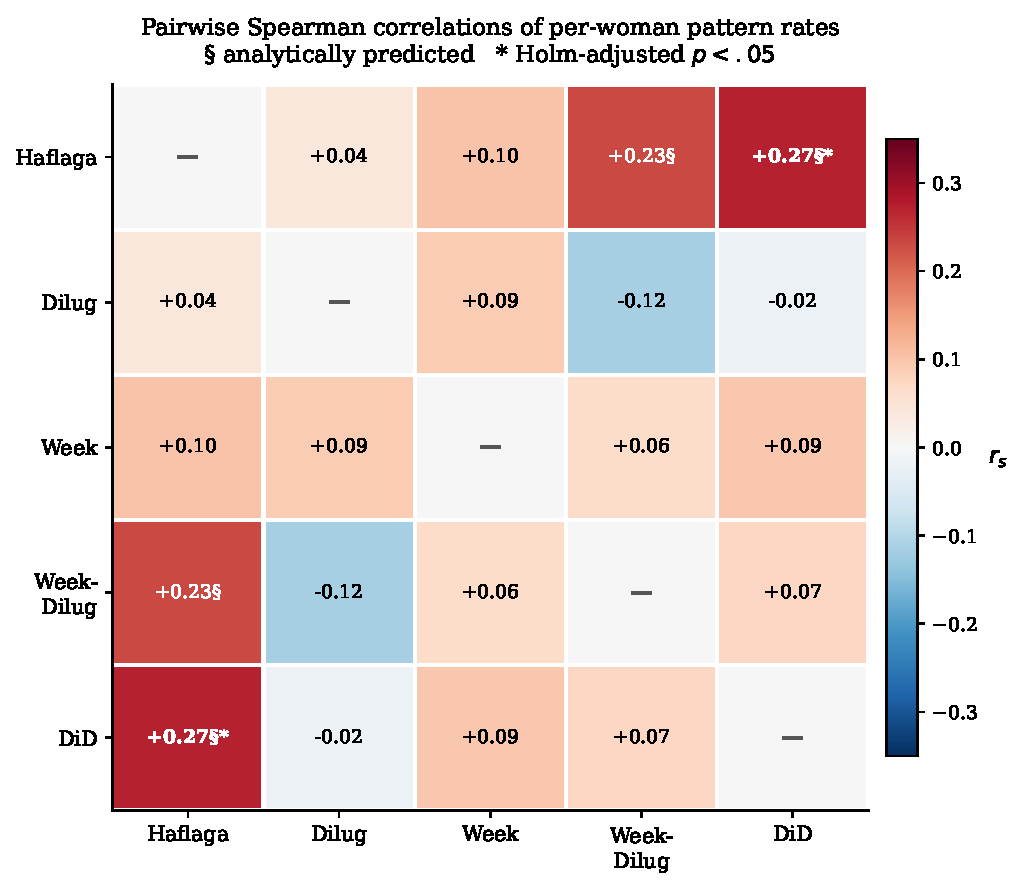
\includegraphics[width=\textwidth]{fig8_chisq_heatmap}
  \caption{Pairwise Spearman correlation structure between vesset pattern types.
    Each cell shows $r_s$ (rate-based Spearman correlation); darker shading
    indicates stronger positive association; lighter shading indicates weaker or
    negative association. Both analytically predicted pairs
    (Haflaga $\times$ Dilug-in-Dilug and Haflaga $\times$ Week-Dilug, marked \S)
    show positive correlation; Haflaga $\times$ Dilug-in-Dilug survives
    Holm correction ($r_s = 0.27$, adj $p = .030$), compatible with the
    polynomial-hierarchy proximity argument of Section~\ref{sec:mathdep}
    (all pairwise tests are exploratory).}
  \label{fig:chisq}
\end{figure}

The primary 5-pattern Mahalanobis joint test is reported in Section~\ref{sec:joint}.
Figure~\ref{fig:joint3panels} provides a geometric illustration of the displacement
of the observed count vector in the exploratory (Haflaga, Week-Dilug, Dilug-in-Dilug) subspace
under all three null models. The three patterns serve as coordinate axes;
the remaining two patterns (Dilug, Week) are encoded by marker size and point shading.

\begin{figure}[H]
  \centering
  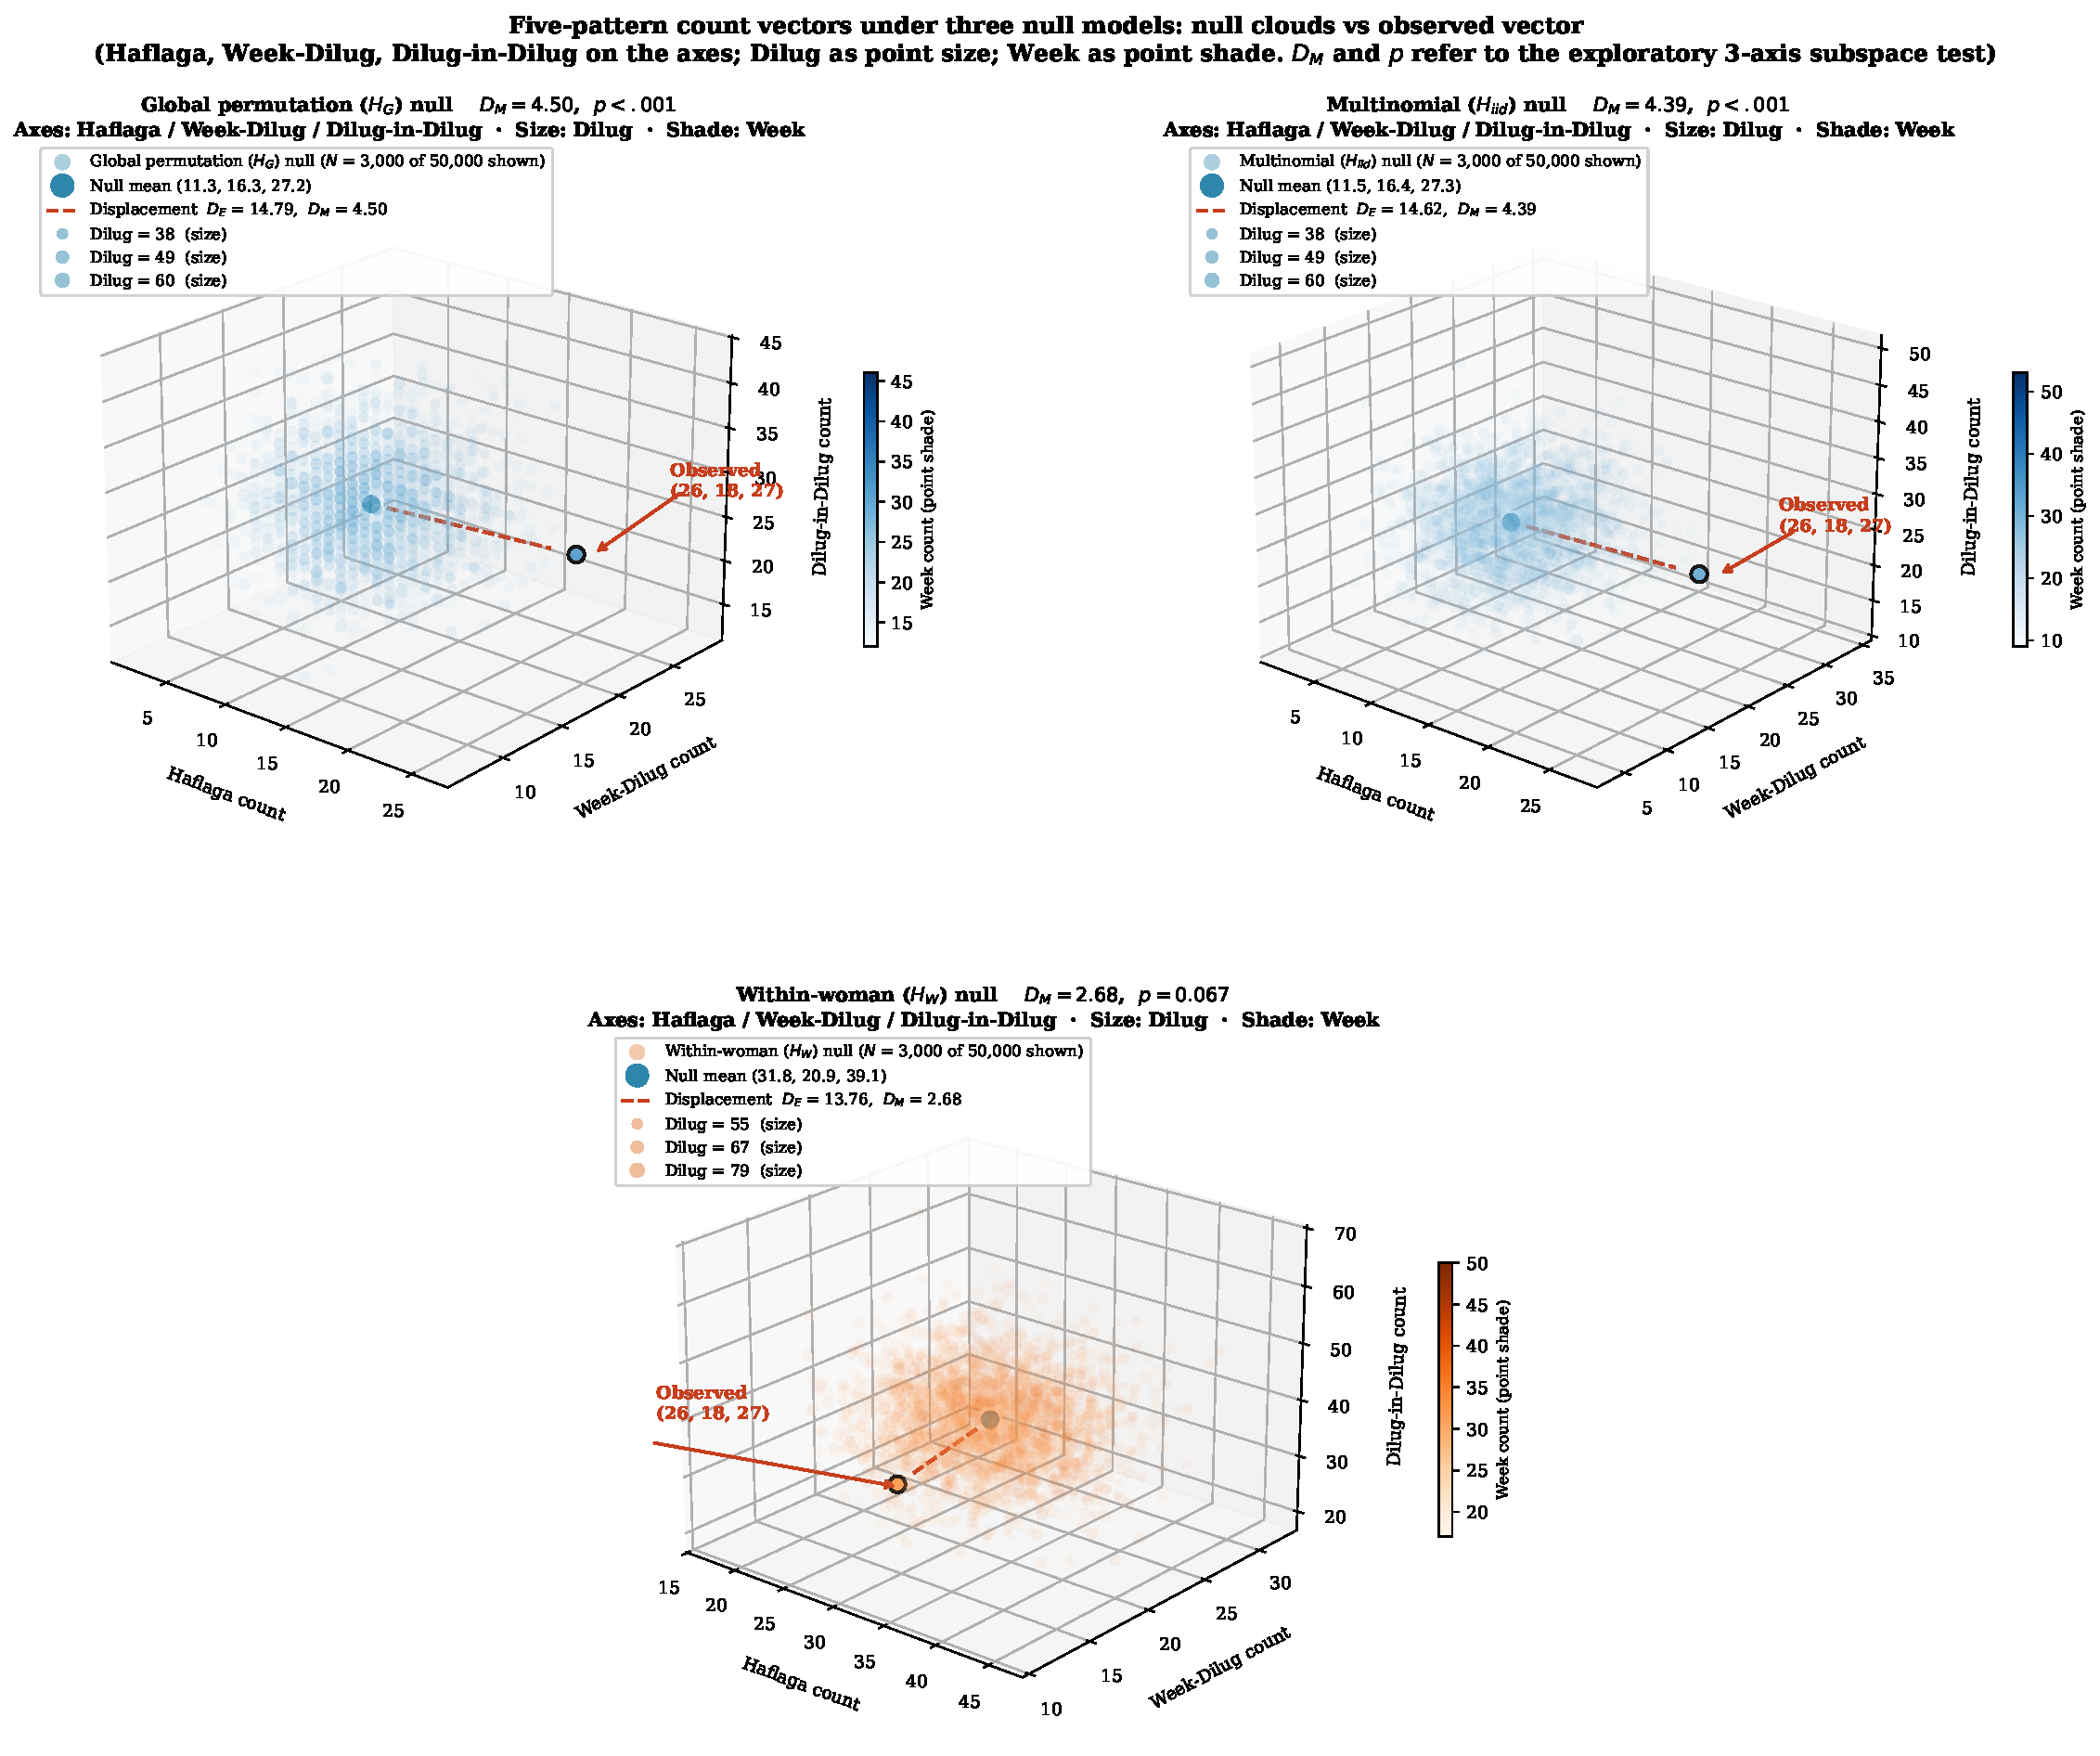
\includegraphics[width=\textwidth]{fig9_joint_3panels}
  \caption{Exploratory focused subspace analysis: displacement of the observed count
    vector $(26, 18, 27)$ in the (Haflaga, Week-Dilug, Dilug-in-Dilug) subspace under the
    \textbf{permutation} ($H_G$, top left), \textbf{multinomial} ($H_{iid}$, top right),
    and \textbf{within-woman} ($H_W$, bottom centre) nulls.
    Marker size encodes Dilug count; marker shading encodes Week count.
    The filled circle marks the null mean; the dashed line identifies the displacement.
    Under $H_G$ and $H_{iid}$ the observed vector lies at the periphery of the null cloud
    (3-pattern $D_M = 4.52$ and $4.36$, both $p < .001$; primary 5-pattern $D_M = 5.10$
    and $4.84$). Under $H_W$ the observed vector falls within the null cloud (3-pattern
    $D_M = 2.68$, $p = .066$; primary 5-pattern $D_M = 2.95$, $p = .121$;
    Table~\ref{tab:stratified}). This figure is an exploratory geometric complement
    to the primary 5-pattern analysis.}
  \label{fig:joint3panels}
\end{figure}

% ─── 5. Discussion ────────────────────────────────────────────────────────────
\section{Discussion}

This study applies a formal permutation-based statistical framework to ask whether halachic vesset
patterns occur at rates distinguishable from chance in empirical menstrual cycle data --- to our
knowledge the first such test applied to this specific domain. The central result is
from the within-woman permutation null ($H_W$): no pattern is individually significant
after Holm correction (all Holm-corrected $p \geq .198$; joint $D_M = 2.95$, $p = .121$), and all observed counts fall
below their within-woman null means. We found no evidence that the temporal ordering
of cycles produces excess vesset-pattern occurrences beyond those expected under
within-woman exchangeability, conditional on each woman's observed cycle-length
multiset. This is a non-detection of excess under the exchangeability null, not a
demonstration that serial dependence is absent: a process with autocorrelation,
latent states, or gradual trends could still fail to reject this particular
permutation null if such structure does not translate into additional exact vesset
events.

\paragraph{Summary of confirmatory vs exploratory results.}
For clarity, we distinguish three categories. \textbf{Pre-specified confirmatory:}
(i) Haflaga overrepresentation under the global null ($p < .001$ after Holm correction);
(ii) the non-significant $H_W$ result (all Holm-corrected $p \geq .198$; joint 5-pattern $D_M = 2.95$, $p = .121$);
(iii) the 5-pattern Mahalanobis joint test under the global null ($D_M = 5.10$, $p < .001$).
\textbf{Exploratory:} Dilug ($p = .087$, Holm adj $p = .346$; hypothesis-generating only), pairwise dependence tests, and the focused 3-pattern subspace analysis (geometric visualization of the structurally dependent triad).
\textbf{Robustness checks:} multinomial null, confirming the global results are not sensitive to null model choice.

Under the global permutation null, which pools cycles across all 118 women,
\textit{Haflaga} is strongly overrepresented ($z = 4.51$, $p < .001$ after
Holm correction) and \textit{Dilug} is not significant ($p = .087$, Holm adj $p = .346$). The joint Mahalanobis test under the global null confirms
significant displacement ($D_M = 5.10$, $p < .001$), driven primarily by Haflaga.
The global overrepresentation reflects concentration of patterns among women who are
intrinsically more regular --- a population-level heterogeneity effect, not evidence
of within-woman temporal structure.

\subsection{Pattern-Specific Findings}

The Haflaga finding is the most striking result. With only 2 of 50,000 permutation
simulations reaching or exceeding the observed count of 26 (the simulation ceiling),
the result is highly significant under the global null and consistent with the
expectation that Haflaga would be concentrated among women with lower within-person
cycle-length variability in this single non-Jewish NFP dataset. Women who establish
Haflaga have within-person SDs of 1.54 days ($n = 20$) vs.\ 3.17 days for women
who establish no vesset at all ($n = 35$; Mann--Whitney $p < .001$, Cohen's
$d = -1.13$; see Section~\ref{sec:data}). Forecasting performance and
generalisability to other populations remain to be evaluated in future work.

The Dilug finding ($p = .087$ under the global null) does not approach significance
and does not survive Holm--Bonferroni correction (adjusted $p = .346$); it should be
treated as hypothesis-generating, requiring pre-registered replication in larger
samples. The direction is consistent with arithmetic progressions arising from
gradual biological trends (e.g., hormonal change, ageing, or weight change), but
these explanations are speculative and await independent confirmation.

\subsection{Mathematical Dependence Structure as a Unifying Observation}

A distinctive feature of this study is that two of the structural relationships between
pattern types derive from the pattern definitions themselves (Section~\ref{sec:mathdep}).
These should be distinguished carefully: one is a strict logical necessity, the other
an algebraic approximation. To our knowledge, this distinction has not previously been
stated explicitly in the halachic or statistical literature.

The three key relationships are: (i)~\textbf{deterministic containment} --- every Haflaga-30
sequence is also a Week-Dilug event by set-theoretic inclusion, so 3 of the 26 Haflaga
cases count deterministically towards Week-Dilug; (ii)~\textbf{algebraic proximity}
--- a Dilug-in-Dilug sequence with small second difference $|d| = 1$ deviates from
a constant sequence by at most a few days, placing it behaviourally close to Haflaga;
this is an algebraic approximation, not a logical implication (the bound depends on
both $|b|$ and $|d|$, so a large first difference can produce substantial variation
even with $|d| = 1$); 16 of the 27 observed DiD sequences have $|d| = 1$, and the
positive association ($\chi^2 = 9.99$, $p_{\text{perm}} = .004$) is consistent with
but not entailed by this proximity; (iii)~\textbf{mutual exclusion at the
window level} --- a cycle pair cannot simultaneously satisfy Dilug ($\Delta^1 H \neq 0$)
and Week-Dilug ($\Delta^1 H = 0$), producing the observed negative direction for
that pair ($p = .300$, non-significant at the woman level).

The five pattern counts are therefore non-independent by construction. The Holm--Bonferroni and joint Mahalanobis procedures answer different inferential questions (FWER control vs.\ a single global null), and the focused 3-pattern Mahalanobis test accounts for the inter-pattern covariance structure through $\hat{\Sigma}^{(3)}$.

\subsection{The Joint Multivariate Test}

The joint test (Eq.~\ref{eq:mahalanobis}) standardises deviations by the full null
covariance $\hat{\Sigma}$, accounting for inter-pattern correlations (condition numbers
4.4--5.4; all pairwise $|r| < 0.16$; see Section~\ref{sec:methods} for full details).
Haflaga has the smallest null SD (3.26 vs.\ 6.60 for Dilug), so its deviation
$(26 - 11.30) = 14.7$ units yields the largest standardised contribution.

The primary 5-pattern Mahalanobis test yields $D_M = 5.10$ ($p < .001$;
0 of 50,000 null replicates exceeded the observed $D_M$) under the permutation null
and $D_M = 4.84$ ($p < .001$; 0 of 50,000 exceeded) under the multinomial null.
An exploratory focused 3-pattern analysis (Haflaga, Week-Dilug, Dilug-in-Dilug)
yields $D_M = 4.52$ ($p < .001$, permutation; 1 of 50,000 exceeded) and $D_M = 4.36$
($p < .001$, multinomial; 0 of 50,000 exceeded), consistent with the primary result.
Haflaga receives appropriately up-weighted contribution via the Mahalanobis metric,
reflecting its larger standardised excess ($z = 4.51$).

\paragraph{Simulation algorithm.}
The covariance matrix $\hat{\Sigma}$ is estimated once per null model from the same
$B = 50{,}000$ simulated count vectors. The same fixed $\hat{\mu}$ and
$\hat{\Sigma}$ are then used to evaluate the Mahalanobis statistic for every null
replicate (a fully Monte Carlo reference distribution, not a leave-one-out
procedure). The observed count vector is not included in $\hat{\mu}$ or
$\hat{\Sigma}$. This procedure is computationally equivalent for all three null models
and yields a purely empirical p-value without parametric assumptions.

This approach is inspired by King et al.\ \cite{king2018} and related to
energy-distance tests \cite{szekely2013} and multivariate permutation tests
\cite{pesarin2010}, but differs in using Mahalanobis distance from the simulated
null mean --- requiring no density estimation, pairwise distances, or asymptotic
approximations. The p-value is purely empirical. A formal theoretical treatment is
planned in future work.

\paragraph{Relationship to Hotelling's $T^2$ and max-$T$.}
The test statistic $D_M^2$ uses the same quadratic form as Hotelling's $T^2$, but
the observed value is evaluated against the empirical null distribution of $D_M$
under permutation, not against a parametric reference distribution. Asymptotic
arguments (e.g., $D_M^2 \approx \chi^2(5)$ under Gaussian approximation) serve as
heuristic background only; the actual inference is entirely distribution-free. With
observed counts as small as 18 (Week-Dilug), the asymptotic approximation is not
relied upon; moreover, Hotelling's $T^2$ additionally assumes multivariate normality
of the test statistic --- an assumption violated by small integer counts such as those
here --- so the parametric form is inappropriate for this application.
The max-$T$ procedure, which bases inference on the single most extreme component
z-score, is less sensitive than Mahalanobis when multiple patterns are simultaneously
displaced from the null; in our data, the two approaches lead to the same substantive
conclusion under both null models.
The Bonferroni--Holm correction and the joint Mahalanobis test answer
different inferential questions: Holm provides family-wise error rate control across
five separate component hypotheses; the Mahalanobis statistic tests a single global
multivariate null. The joint test does not replace Holm, nor is it uniformly more
powerful; it aggregates correlated evidence into one distance measure that is
sensitive to departure in any direction from the null centre.

\subsection{Non-Significant Patterns}

Week, Week-Dilug, and Dilug-in-Dilug were not individually significant. These results
do not invalidate these halachic rules, which are established on legal-theological
grounds \cite{anon2021statistical}. The non-significance of Dilug-in-Dilug is
particularly notable given its large z-score at the sequence level in the joint test:
it is the dependence with Haflaga (via the polynomial hierarchy) that elevates its
collective contribution to $D$, even when its individual count is exactly at the null
mean. This illustrates why joint and individual tests can differ.

For the Week pattern, it is worth noting that the weekly anchor set
$\mathcal{W} = \{22, 29, 36, 43, 50\}$ (in haflaga units) corresponds to cycle lengths
$\{21, 28, 35, 42, 49\}$. Since cycles of 35 days or longer are uncommon in the Fehring dataset
(9.6\% of all cycles; mean $L = 29.3$, SD $= 3.9$), nearly all
Week patterns in this sample arise from haflaga values of 22 (cycle length 21) or 29
(cycle length 28). The 28-day cycle is the mode of the dataset and the most
biologically common length, so the Week pattern in this dataset effectively captures
women with near-28-day cycles who also show the requisite two-consecutive-cycle
consistency.

\subsection{Clinical and Halachic Implications}

The findings carry several implications, all of which should be understood as
hypotheses for future study rather than clinical guidance: none of the outcomes
discussed below is directly evaluated in the present analysis.

\paragraph{Fertility awareness.}
Women with established Haflaga represent the most cycle-regular subgroup in this
dataset (within-person SD: 1.54 days vs.\ 3.17 days for non-vesset women). For such
women, backward estimation of the fertile window (approximately 14 days prior to
anticipated onset) is most reliable, making Haflaga a candidate marker for
calendar-based fertility planning \cite{bortot2010}. Whether this marker improves
on statistical cycle-length prediction methods will be examined in the companion
forecasting study \cite{anon_planned}.

\paragraph{Halachic family purity compliance.}
For observant Jewish women, the vesset system governs the timing of ritual abstinence
(\textit{taharat hamishpacha}). The finding that Haflaga is associated with lower observed cycle-length variability
motivates evaluation of vesset-derived features as candidate markers of cycle
regularity in prospective studies; a direct comparison with established
cycle-forecasting methods remains a topic for future work.
The non-significance under the within-woman null is consistent with the halachic
position that vesset rules codify observed regularity rather than impose temporal
structure beyond it. Whether these empirical
findings bear on the legal-theological validity of vesset rules is a question outside the scope of this analysis.

\paragraph{Cycle regularity as a health indicator.}
Menstrual cycle irregularity is associated with decreased fertility and elevated risk
of chronic conditions \cite{bortot2010}. The finding that Haflaga marks women with
low within-person cycle-length variability (SD $< 1.6$ days) suggests it could
function as a simple regularity indicator --- a clinical hypothesis to be evaluated
in datasets with longitudinal clinical measurements and defined clinical endpoints.
Changes in vesset status (loss or gain of Haflaga) may also serve as a signal of
disruption to baseline regularity, warranting prospective investigation.

\subsection{Scope and Generalizability}

Before discussing specific limitations, we emphasise that all conclusions are
restricted to this specific dataset of non-Jewish NFP users. The results should
not be generalised to the general population or to observant Jewish women without
replication. The NFP dataset represents a self-selected group of cycle-aware women,
likely more regular than the general population, which may inflate pattern counts.
Any inference about the halachic validity of vesset rules in the Jewish context
requires datasets collected from the target population.
Such validation within an observant Jewish demographic would directly bridge the
statistical findings to their halachic application context.

\subsection{Limitations}
\label{sec:limitations}

\paragraph{Data quality and coding.}
The haflaga convention $H_k = L_k + 1$ is a conventional relabelling; pattern counts
are identical whether computed on $H_k$ or $L_k$ \emph{provided the anchor shifts by the
same $-1$} (verified: Haflaga 26, Week-Dilug 18 under both conventions).
Computing on $L_k$ with the unadjusted anchor ($L = 30$ instead of $L = 29$) yields
only 12 Week-Dilug events instead of the correct 18.
As a sensitivity diagnostic, the raw haflaga distribution was inspected for heaping
artefacts at round numbers. Counts decline smoothly from the mode ($H = 29$: 225
cycles) through the Week-Dilug anchor ($H = 30$: 175) to $H = 31$ (141); this
pattern is consistent with the known biological mode at 29--30 days rather than
digit rounding (Figure~\ref{fig:heaping}). This diagnostic is descriptive; a formal
statistical test for digit preference is not performed.
The NFP dataset records cycle length in whole days but not onset time of day, creating
potential misclassification relative to the halachic requirement that all pattern
onsets occur in the same onset period (daytime or nighttime). Both upward and downward
biases are possible; their relative magnitude cannot be assessed, but the effect is
expected to be approximately uniform across women and pattern types. If menstruation onset timing varies systematically with individual physiology, misclassification could differ across women; however, the within-woman null ($H_W$) conditions on each woman's observed cycle-length multiset, so any consistent within-woman shift in recorded lengths is preserved identically across observed and permuted sequences, leaving the $H_W$ test unaffected by this form of individual-level misclassification.

\paragraph{Dataset scope.}
Calendar dates are absent, precluding analysis of the 10 date-dependent vesset types;
two of the 7 cycle-length types (Dilug Chozer Chalila, Haflaga Chozer Chalila) had
zero occurrences due to their stringent run-length requirements, leaving the 5
patterns analysed here. The dataset also excludes prodromal physical symptoms
(\textit{vesset haguf}): women may have established body-sign vesset patterns
entirely invisible to cycle-length analysis.

\paragraph{Population generalizability.}
Participants are non-Jewish NFP users \cite{fehring2013}: regularly cycling married
women aged 18--42. NFP users are a self-selected group likely more cycle-aware and
possibly more regular than the general population, introducing a potential upward bias
in regularity-dependent patterns such as Haflaga. Several halachic authorities hold
that regularities in non-Jewish women may not generalise to Jewish women in practice
\cite{anon2022phd}.

\paragraph{Statistical methodology.}
The global null models ($H_G$, $H_{\text{iid}}$) shuffle cycle lengths across women,
ignoring within-person autocorrelation; $H_W$ addresses this by conditioning on each
woman's own cycle-length distribution, but tests only the specific exchangeability
null that all orderings of a woman's observed multiset are equally probable --- not
a general test of serial independence or stationarity. Future work could employ
parametric nulls based on fitted state-space models \cite{bortot2010,symul2019}.
The pairwise rate-based analysis mitigates the cycle-count exposure confound by
normalising event counts by the number of cycles per woman; associations involving
rare patterns (Week-Dilug: 18 events; Dilug-in-Dilug: 27 events) should nonetheless
be interpreted as exploratory, given the limited number of women establishing those
patterns. The Haflaga $\times$ Dilug-in-Dilug association that survives Holm correction
is further supported by the polynomial-proximity argument (Section~\ref{sec:mathdep}),
providing structural justification beyond the empirical correlation.
As an approximate sensitivity benchmark, we computed a minimum detectable count (MDC)
for each pattern under $H_W$, quantifying the minimum count that would be detectable
at $\alpha = .05$ (two-sided) with 80\% sensitivity under a normal-theory location-shift approximation:
\begin{equation}
  \text{MDC} \approx \mu_W + (z_{0.025} + z_{0.80})\,\sigma_W
             = \mu_W + 2.802\,\sigma_W.
\end{equation}
MDC values are normal-theory effect-size benchmarks --- approximate positive-shift sensitivity thresholds, not
exact power guarantees or evidence of the study being underpowered in a prospective sense
(Table~\ref{tab:power}); a simulation-based sensitivity analysis is deferred to future work.
All five observed counts fall below their MDC, indicating that effects of the magnitude
studied here would require a larger dataset to detect reliably at this sensitivity level;
the joint $H_W$ test is likewise non-significant ($D_M = 2.95$, $p = .121$).

\begin{figure}[H]
  \centering
  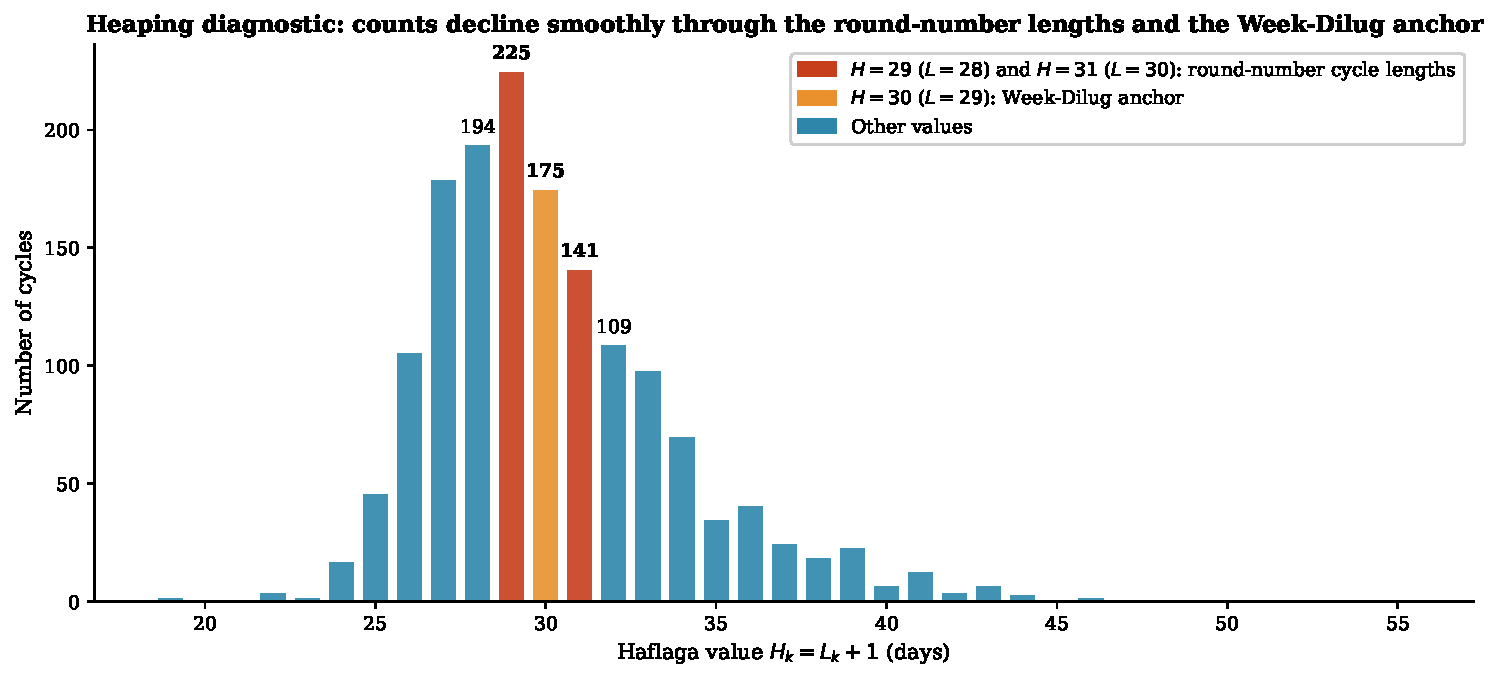
\includegraphics[width=0.88\textwidth]{figA1_heaping_diagnostic}
  \caption{Distribution of haflaga values $H_k$ around $H = 28$ and $H = 30$.
    The distribution is smooth with no heaping artefact at $H = 30$
    ($H = 29$: 225 cycles; $H = 30$: 175; $H = 31$: 141), confirming that the
    Week-Dilug anchor at $H = 30$ does not reflect a reporting bias.}
  \label{fig:heaping}
\end{figure}

\begin{table}[ht]
\centering
\caption{Approximate detectable-count benchmarks under $H_W$ (within-woman permutation null),
  based on a normal-theory location-shift approximation.
  $\mu_W$: null mean; $\sigma_W$: null SD; 95th pct: empirical 95th percentile
  of null (rejection threshold at $\alpha = .05$); MDC: minimum detectable count
  at nominal 80\% sensitivity ($\text{MDC} \approx \mu_W + 2.802\,\sigma_W$, where
  $z_{0.025} + z_{0.80} = 1.960 + 0.842 = 2.802$; approximate normal-theory benchmark, not an exact power guarantee); $z_{\text{obs}}$: standardised
  observed count.
  All observed counts fall below the MDC, consistent with limited sensitivity
  at $N = 118$.}
\label{tab:power}
\begin{tabular}{lrrrrrrr}
\hline
Pattern & Obs.\ & $\mu_W$ & $\sigma_W$ & 95th pct & MDC & $z_{\text{obs}}$ \\
\hline
Haflaga        & 26 & 31.85 & 4.68 & 40.0 & 45 & $-1.25$ \\
Dilug          & 61 & 67.07 & 7.36 & 79.0 & 88 & $-0.83$ \\
Week           & 32 & 33.81 & 3.88 & 40.0 & 45 & $-0.47$ \\
Week-Dilug     & 18 & 20.94 & 3.22 & 26.0 & 30 & $-0.91$ \\
Dilug-in-Dilug & 27 & 39.14 & 5.86 & 49.0 & 56 & $-2.07$ \\
\hline
\end{tabular}
\end{table}

% ─── 6. Conclusion ────────────────────────────────────────────────────────────
\section{Conclusion}

This study applies a formal permutation-based statistical framework to ask whether halachic vesset
patterns occur at rates distinguishable from chance in empirical menstrual cycle data --- to our
knowledge the first such analysis applied to this specific domain. The five patterns
analysed form a polynomial hierarchy whose structure generates algebraic structural
relationships --- one a strict logical containment (Haflaga-30 $\subseteq$ Week-Dilug),
one an algebraic approximation (Haflaga--Dilug-in-Dilug proximity) --- explored
through exploratory pairwise randomisation-based tests. Three complementary null
models were applied: a global permutation null, a multinomial null, and the
scientifically sharper within-woman permutation null ($H_W$).

The primary result is from the within-woman null: under $H_W$, \emph{no pattern is
individually significant} (all Holm-corrected $p \geq .198$; joint $D_M = 2.95$, $p = .121$), and
all observed counts fall below their within-woman null means. These findings provide no evidence, under within-woman exchangeability, that
temporal ordering within each woman's cycle sequence creates vesset patterns
beyond what her own cycle-length distribution predicts. This is a non-detection of excess under the exchangeability null; all five observed counts fall below the normal-theory sensitivity benchmark (Table~\ref{tab:power}), indicating that effects of this magnitude would require a larger dataset to detect reliably. This result should be interpreted as no detectable evidence of within-woman temporal structure under this null, not as proof of its absence.

Under the global null, Haflaga is significantly overrepresented ($p < .001$ after
Holm correction); Dilug is not significant ($p = .087$, Holm adj $p = .346$) and should be treated as hypothesis-generating pending
replication. The joint Mahalanobis test confirms significant displacement from the
global null ($D_M = 5.10$, $p < .001$; only 2 of 50,000 permutation simulations
reached the observed Haflaga count). This global result is best interpreted as a
descriptive decomposition: it demonstrates that women who establish Haflaga are
drawn from a subpopulation with lower cycle-length variability, a population-level
heterogeneity effect that does not, by itself, constitute evidence of within-woman
temporal predictability. The primary 5-pattern Mahalanobis joint test yields $D_M = 5.10$, $p < .001$
under the global null, driven primarily by Haflaga. An exploratory focused analysis
restricted to the three structurally dependent patterns (Haflaga, Week-Dilug,
Dilug-in-Dilug) yields $D_M = 4.52$, $p < .001$, consistent with the primary result. Together, these results suggest that halachic vesset rules function
primarily as empirical detectors of individual cycle regularity: the rules identify
the subset of women with lower observed cycle-length variability and formalise that
regularity as an anticipatory pattern. The joint distance-based permutation test, adapted here for dependent count vectors
in sequential menstrual-cycle data (conceptually related to quadratic-form and
energy-distance permutation tests; see Section~\ref{sec:joint}), provides a way to
aggregate correlated count evidence into a single global multivariate null test.
The Holm--Bonferroni correction and the joint Mahalanobis test answer different
inferential questions --- Holm controls FWER across five separate hypotheses, while
the Mahalanobis statistic tests one global null --- and the two procedures are
complementary rather than competing. This adapted approach may prove useful for
composite hypothesis testing in other cyclic biological settings (e.g., multitype
rhythm patterns, circadian or hormonal cycle data, episodic clinical event sequences)
where structurally related count outcomes are tested jointly.


% ─── AI Disclosure ────────────────────────────────────────────────────────────
\section*{AI Assistance Disclosure}

Portions of the written text in this article were drafted and edited with the
assistance of Claude (Anthropic, 2024), a large language model AI assistant.
All scientific content, mathematical derivations, statistical analyses, and
intellectual contributions are solely the work of the author. The AI tool was
used exclusively for language editing, structural organisation of the manuscript,
and generation of \LaTeX{} and Python code under the author's direct supervision
and verification. The author takes full responsibility for the accuracy and
integrity of all content presented in this article.

% ─── References ───────────────────────────────────────────────────────────────
\newpage
\bibliographystyle{unsrtnat}
\bibliography{references}

\end{document}
